% Set document class
\documentclass[hidelinks,12pt]{article}

% Define packages
\usepackage{hyperref, url} 
\usepackage{graphicx,amsfonts,psfrag,layout,subcaption,array,longtable,lscape,booktabs,dcolumn,amsmath,amssymb,amssymb,amsthm,setspace,epigraph,chronology,color,colortbl,wasysym,diagbox,natbib,colortbl,authblk,commath,upgreek}
\usepackage[]{graphicx}\usepackage[]{color}
\usepackage[page]{appendix}
\usepackage[section]{placeins}
\usepackage[linewidth=1pt]{mdframed}
\usepackage[margin={1in}]{geometry} %1 inch margins

% Telephone code
\def\Plus{\texttt{+}}
\def\Minus{\texttt{-}}

\title{RNN-Based Counterfactual Prediction} 
\author[ ]{Jason Poulos\thanks{PhD Candidate, Department of Political Science, 210 Barrows Hall \#1950, Berkeley, CA 94720-1950. \emph{Email:} \href{mailto:poulos@berkeley.edu}{\nolinkurl{poulos@berkeley.edu}}. \emph{Telephone:} \Plus 1\Minus 510\Minus 642\Minus 6323. I acknowledge support of the National Science Foundation Graduate Research Fellowship (DGE 1106400). This work used the computer resources of Stampede2 at the Texas Advanced Computing Center (TACC) under an Extreme Science and Engineering Discovery Environment (XSEDE) startup allocation (TG-SES180010). The Titan Xp GPU used for this research was donated by the NVIDIA Corporation.}}
\affil[ ]{University of California, Berkeley}
\date{}
\setcounter{Maxaffil}{0}
\renewcommand\Affilfont{\itshape\small}

\usepackage[autosize]{dot2texi}
\usepackage{tikz}
\usetikzlibrary{shapes,arrows}

%% Centered and capitalized section headings
%
%\usepackage{sectsty}
%\sectionfont{\centering\normalfont\scshape}

% Reference labels in the online appendix
%\usepackage{xr}
%\externaldocument{rnns-causal-sm}

% Footnotes stick at the bottom
\usepackage[bottom]{footmisc}

% Caption keys
\usepackage{mathtools,tikz,caption}
\captionsetup{labelfont=sc,labelsep=period}
\DeclareRobustCommand\sampleline[1]{%
	\tikz\draw[#1] (0,0) (0,\the\dimexpr\fontdimen22\textfont2\relax)
	-- (2em,\the\dimexpr\fontdimen22\textfont2\relax);%
}

\usetikzlibrary{plotmarks}

% Multicolumns for references
\usepackage{multicol}

% Wes Anderson colors

\usepackage{xcolor}

\definecolor{Darjeeling11}{HTML}{FF0000}
\definecolor{Darjeeling15}{HTML}{5BBCD6}

% New footnote characters
\usepackage{footmisc}
\DefineFNsymbols{mySymbols}{{\ensuremath\dagger}{\ensuremath\ddagger}\S\P
	*{**}{\ensuremath{\dagger\dagger}}{\ensuremath{\ddagger\ddagger}}}
\setfnsymbol{mySymbols}

%Rm thanks dagger
\renewcommand\footnotemark{}
%\renewcommand\footnoterule{}

% New tabular environment
\usepackage{tabularx}
\newcolumntype{Y}{>{\raggedleft\arraybackslash}X}% raggedleft column X

% Define appendix 
\renewcommand*\appendixpagename{Appendix}
\renewcommand*\appendixtocname{Appendix}

% Position floats
\renewcommand{\textfraction}{0.05}
\renewcommand{\topfraction}{0.95}
\renewcommand{\bottomfraction}{0.95}
\renewcommand{\floatpagefraction}{0.35}
\setcounter{totalnumber}{5}

% Colors for highlighting tables
\definecolor{Gray}{gray}{0.9}

% Different font in captions
\newcommand{\captionfonts}{\normalsize}

\makeatletter  % Allow the use of @ in command names
\long\def\@makecaption#1#2{%
	\vskip\abovecaptionskip
	\sbox\@tempboxa{{\captionfonts #1: #2}}%
	\ifdim \wd\@tempboxa >\hsize
	{\captionfonts #1: #2\par}
	\else
	\hbox to\hsize{\hfil\box\@tempboxa\hfil}%
	\fi
	\vskip\belowcaptionskip}
%\makeatother   % Cancel the effect of \makeatletter

% Set Spacing
\doublespacing

% Number assumptions
\newtheorem*{assumption*}{\assumptionnumber}
\providecommand{\assumptionnumber}{}
\makeatletter
\newenvironment{assumption}[2]
{%
	\renewcommand{\assumptionnumber}{Assumption #1}%
	\begin{assumption*}%
		\protected@edef\@currentlabel{#1}%
	}
	{%
	\end{assumption*}
}
\makeatother

% Macros
\newcommand{\Adv}{{\boldsymbol{Adv}}}       
\newcommand{\prp}{{\mathrm{prp}}}                  % How to define new commands 
\newcommand{\calK}{{\cal K}}
\newcommand{\outputs}{{\Rightarrow}}                
\newcommand{\getsr}{{\:\stackrel{{\scriptscriptstyle\hspace{0.2em}\$}}{\leftarrow}\:}}
\newcommand{\andthen}{{\::\;\;}}    %  \: \; for thinspace, medspace, thickspace
\newcommand{\Rand}[1]{{\mathrm{Rand}[{#1}]}}       % A command with one argument
\newcommand{\Perm}[1]{{\mathrm{Perm}[{#1}]}}       
\newcommand{\Randd}[2]{{\mathrm{Rand}[{#1},{#2}]}} % and with two arguments
\newcommand{\E}{\mathrm{E}}
\newcommand{\Var}{\mathrm{Var}}
\newcommand{\Cov}{\mathrm{Cov}}
\DeclareMathOperator*{\plim}{plim}
\newcommand\independent{\protect\mathpalette{\protect\independenT}{\perp}}
\def\independenT#1#2{\mathrel{\rlap{$#1#2$}\mkern2mu{#1#2}}}
\newcommand{\possessivecite}[1]{\citeauthor{#1}'s (\citeyear{#1})} 
\DeclareMathOperator*{\argmin}{arg\,min}

%%%%%%%%%%%%%%%%%%%%%%%%%%%%%%%%%%%%%%%%%%%%%%%%%%%%%%%%%%%%%%%%%%%%%%%%%%%%

\begin{document} 
 
\begin{singlespacing}
\maketitle  
\end{singlespacing}
\thispagestyle{empty}

\pagenumbering{roman}% Roman-numbered pages (start from i)
\begin{abstract}  % abstract of 150 to 250 words
\noindent 
This paper proposes an alternative to the synthetic control method (SCM) for estimating the effect of a policy intervention on an outcome over time. Recurrent neural networks (RNNs) are used to predict counterfactual time-series of treated units using only the outcomes of control units as model inputs. The proposed method does not rely on pre-intervention covariates to construct the synthetic control and is consequently less susceptible to $p$-hacking. RNNs are also capable of handling multiple treated units and can learn nonconvex combinations of control units. In placebo tests, RNNs outperform the SCM in predicting the post-intervention time-series of control units, while yielding a comparable proportion of false positives. The RNN-based approach contributes to a new generation of data-driven machine learning techniques such as matrix completion and the Lasso for generating counterfactual predictions.
\\
\begin{singlespace}
	\emph{Keywords:} Counterfactual Prediction; Recurrent Neural Networks; Randomization Inference; Synthetic Controls; Time-Series Cross-Section Data
\end{singlespace}
\end{abstract}

%Move introduction to second page
\pagebreak
\pagenumbering{arabic}% Arabic-numbered pages (start from 1)

\section{Introduction} 

An important problem in the social sciences is estimating the effect of a binary intervention on an outcome over time. When interventions take place at an aggregate level (e.g., a state), researchers make causal inferences by comparing the post-intervention (``post-period'') outcomes of affected (``treated'') units against the outcomes of unaffected  (``control'') units. A common approach to the problem is the synthetic control method (SCM) \citep{abadie2010synthetic}, which predicts the counterfactual outcomes of treated units by finding a convex combination of control units that match the treated units in term of lagged outcomes. Correlations across units are assumed to remain constant stable time. 

The SCM has several limitations. First, the convexity restriction of the synthetic control estimator precludes dynamic, nonlinear interactions between multiple control units. Intuitively, one can expect that the treated unit may exhibit nonlinear or negative correlations with the control units. \citet{ferman2016revisiting} demonstrate that the convexity restriction implies that the SCM estimator may be biased even if selection into treatment is only correlated with time-invariant unobserved covariates. Second, \citet{ferman2018synthetic} demonstrate that the SCM is generally biased if treatment assignment is correlated with unobserved confounders, even when the number of pre-intervention periods grows \citep{ferman2018synthetic}. Moreover, the authors show that while the SCM minimizes imbalance in pre-period outcomes, the likelihood of finding exact balancing weights vanishes as the number of time periods increase, which results in bias. 

While the strength of the SCM lies in its simplicity in setup and implementation, several problems arise from the lack of guidance on how to specify the SCM estimator. The specification of the estimator can produce very different results: \citet{ferman2018cherry} show, for example, how cherry-picking between common SCM specifications can facilitate $p$-hacking.\citet{kaul2015synthetic} show that the common practice of including lagged versions of the outcome variable as model inputs can render all other covariates irrelevant. \citet{klossner2017comparative} demonstrates that the common practice of using cross-validation to select importance weights can yield multiple values and consequently different results. 

This paper proposes an alternative to the SCM that is capable of automatically selecting appropriate control units at each time-step, allows for nonconvex combinations of control units, and does not rely on pre-intervention covariates. The method uses recurrent neural networks (RNNs) to predict a counterfactual time-series of treated units using only control unit outcomes as model inputs. RNNs are a class of neural networks that take advantage of the sequential nature of time-series data by sharing model parameters across multiple time-steps \citep{el1995}. Non-parametric models such as RNNs are useful for prediction problems because we do not have to assume a functional form on the data. In addition, RNNs can learn the most useful nonconvex combination of control unit outcomes at each time-step for generating counterfactual predictions. Relaxing the convexity restriction is useful when the data-generating process underlying the outcome of interest depends nonlinearly on the history of its inputs. RNNs have been shown to outperform various linear models on time-series prediction tasks \citep{cinar2017position}. 

The proposed method builds on a new literature that uses machine learning methods for data-driven synthetic controls, such as matrix completion \citep{athey2017matrix,2019arXiv190308028P}, or two-stage estimators that reduces data dimensionality via L1-regularized regression \citep{doudchenko2016balancing,carvalho2018arco} or matrix factorization \citep{amjad2018robust} prior to regressing the outcomes on the reduced data. These methods are data-driven in the sense that they are capable of finding an appropriate subset of control units for comparison in the absence of domain knowledge or pre-intervention covariates. 

RNNs are end-to-end trainable and very flexible to a given sequential prediction problem. For example, they are capable of sharing learned parameters across time-steps and multiple treated units. while the SCM can be generalized to handle multiple treated units \citep[e.g.,][]{dube2015pooling,xu2017generalized}, the generalized the SCM is not capable of sharing model weights when predicting the outcomes of multiple treated units. Regularization methods such as dropout can easily be incorporated into RNN architectures to prevent overfitting during the training process, which is problematic when the networks learn an overreliance on a few model inputs.

In the section immediately below, I describe the problem of counterfactual prediction and its relationship to matrix completion and the problem of covariate shift; Section \ref{RNNs-section} introduces the approach of using RNNs for counterfactual prediction; Section \ref{placebo} presents the results of the placebo tests; Section \ref{eval} details the procedure for hypothesis testing; Section \ref{schooling-app} applies the RNN-based method and inferential procedure ot the problem of estimating the impact of homestead policy on long-run state government investment in public schooling; Section \ref{conclusion} concludes and offers potential avenues for future research. 

%\setcounter{section}{1}
\section{Counterfactual prediction} \label{prediction}

The proposed method estimates the causal effect of a discrete intervention in observational panel data; i.e., settings in which treatment is not randomly assigned and there exists both pre- and post-period observations of the outcome of interest. Let $\boldsymbol{Y}$ denote a $\text{N} \times \text{T}$ matrix of outcomes for each unit $i =1, \ldots, \text{N}$ at time $t = 1, \ldots, \text{T}$. $\boldsymbol{Y}$ is incomplete because we observe each element $Y_{it}$ for only the control units and the treated units prior to time of initial treatment exposure, $\text{T}_0 < \text{T}$. Let $\mathcal{O}$ denote the set of $(it)$ values that are observed and $\mathcal{M}$ the set of $(it)$ missing values. Let the values of the $\text{N} \times \text{T}$ complete matrix $\boldsymbol{W}$ be $W_{it} =1$ if $(it) \in \mathcal{M}$ and $W_{it} = 0$ if $(it) \in \mathcal{O}$. Note that the process that generates $W_{it}$ is referred to the treatment assignment mechanism in the causal inference literature \citep{imbens2015causal} and the missing data mechanism in missing data analysis \citep{little2014}. The pattern of missing data is assumed to follow from the simultaneous treatment adoption setting, where treated units are exposed to treatment at time $\text{T}_0$ and every subsequent period. 

This setup is motivated by the \citet{neyman1923} potential outcomes framework, where for each $it$ value there exists a pair of potential outcomes, $Y_{it}(1)$ and $Y_{it}(0)$, which represents the response to treated and control regimes, respectively. The observed outcomes are 

\begin{align} 
Y_{it} = \begin{cases}
Y_{it}(0) 	& \mbox{if } W_{it} = 0  \text{ or } t < \text{T}_0 \\
Y_{it}(1) 	& \mbox{if } W_{it} = 1  \text{ and } t \geq \text{T}_0.
\end{cases} 
\end{align} 

The problem of counterfactual prediction is that we cannot directly observe the missing potential outcomes and instead wish to impute the missing values in $\boldsymbol{Y}(0)$ for treated units with $W_{it} =1$.  The potential outcomes framework explicitly assumes unconfoundedness. In an observational setting, this assumption requires $(\boldsymbol{Y}(0), \boldsymbol{Y}(1)) \independent \boldsymbol{W}| \boldsymbol{Y}(\mathcal{O})$, where $\boldsymbol{Y}(\mathcal{O})$ is the observed data. 

The potential outcomes framework also implicitly assumes treatment is well-defined to ensure that each unit has the same number of potential outcomes \citep{imbens2015causal}. It also excludes interference between units, which would undermine the framework by creating more than two potential outcomes per unit, depending on the treatment status of other units \citep{rubin1990}.

\subsection{Relationship to matrix completion and covariate shift}

The proposed approach is similar to the method of matrix completion via nuclear norm minimization (MC-NNM) proposed by \citet{athey2017matrix} to predict counterfactual outcomes. Matrix completion methods attempt to impute missing entries in a low-rank matrix by solving a convex optimization problem via NNM, even when relatively few values are observed in $\boldsymbol{Y}$ \citep{candes2009exact,candes2010matrix}. The estimator recovers a $\text{N} \times \text{T}$ low-rank matrix by minimizing the sum of squared errors via nuclear norm regularized least squares. The estimator reconstructs the matrix by iteratively replacing missing values with those recovered from a singular value decomposition \citep{mazumder2010spectral}. 

\citet{athey2017matrix} note two drawbacks of MC-NNM. First, the errors may be autocorrelated because the estimator does not account for time-series dependencies in the observed data. The estimator estimate patterns row- and column-wise, but treat the data as perfectly synchronized \citep{yoon2018estimating}. In contrast, the RNN-based approach described in Section \ref{RNNs-section} exploits the temporal component of the data and therefore does not have the problem of autocorrelated errors. 

Second, the MC-NNM estimator penalizes the errors for each observed value equally without regard to the fact that the probability of missingness (i.e, the propensity score), increases with $t$. \citet{athey2017matrix} suggest weighting the loss function by the propensity score, which is similar to the importance weighting scheme proposed by \citet{cortes2008sample} to address the problem of covariate shift, which is a special case of domain adaptation \citep{huang2007correcting,ben2007analysis,bickel2009discriminative,cortes2010learning,2015arXiv150507818G}.\footnote{\citet{schnabel2016recommendations} first connected the matrix completion problem with causal inference in observational settings in the context of recommender systems under confounding. \citet{johansson2016learning} formulates the general problem of counterfactual inference as a covariate shift problem.} 

The covariate shift problem occurs when training and test data are drawn from different distributions. For notational ease, define the training set input-output pair as 

$$\left(\boldsymbol{X}^{\text{train}}, \boldsymbol{Y}^{\text{train}}\right) = \left(\boldsymbol{Y}(\boldsymbol{W})^{\{t < \text{T}_0\}}, \boldsymbol{Y}(\boldsymbol{W})^{\{t \geq \text{T}_0\}}\right)$$
\noindent
for units with $\boldsymbol{W}=1$ and the test set pair $\left(\boldsymbol{X}^{\text{test}}, \boldsymbol{Y}^{\text{test}}\right)$ for units with $\boldsymbol{W}=1$. In the proposed approach, the model weights learned on the training set is fit on $\boldsymbol{X}^{\text{test}}$ to predict $\boldsymbol{Y}^{\text{test}}$. The approach therefore assumes similarity between the distributions of $\boldsymbol{X}^{\text{train}}$ and $\boldsymbol{X}^{\text{test}}$. In order to minimize the discrepancy between the training and test set input distributions, I estimate the propensity score $\hat{e_{it}} = \Pr(W_{it}=1 | Z_{it})$, conditional on covariate matrix $\boldsymbol{Z}$ and then weight the training loss by the estimated propensity scores. 

\subsection{Nonparametric regression}

In its most basic form, counterfactual prediction can be represented as a nonparametric regression,

\begin{equation}\label{eq:np}
  \boldsymbol{\hat{\boldsymbol{Y}}^{\text{train}}} =  \hat{f_0} \left(\boldsymbol{X}^{\text{train}}\right) + \upepsilon^{(t)},
\end{equation}
\noindent
where the noise variables $\epsilon^{(t)}$ are assumed to be i.i.d. standard normal and independent of the observed data. The nonlinear function $\hat{f_0}$ is estimated by minimizing the weighted mean squared error, 

\begin{equation} \label{eq:mse}
\text{W-MSE} = \E \left[\left(\boldsymbol{Y}^{\text{train}} - \boldsymbol{\hat{Y}}^{\text{train}}  \right)^2 \right]  \boldsymbol{\hat{E}}^\text{train},
\end{equation}
\noindent
where $\boldsymbol{\hat{E}}^\text{train}$ is a matrix of estimated propensity scores of the same dimension as $\boldsymbol{X}^\text{train}$. 

At test time, the estimated function is used to predict $\boldsymbol{\hat{Y}}^{\text{test}} = \hat{f_0} \left(\boldsymbol{X}^{\text{test}}\right)$. The estimated causal effect of the intervention is then

\begin{equation}\label{eq:pointwise}
  \boldsymbol{\hat{\phi}} = \boldsymbol{Y}^{\text{test}} - \boldsymbol{\hat{Y}}^{\text{test}}. 
\end{equation}

This treatment effect is calculated at every post-period time-step and is thus useful for understanding the temporal evolution of the causal effect.

\section{RNNs for counteractual prediction} \label{RNNs-section}

RNNs \citep{graves2012,goodfellow2016deep} consist of an input $\boldsymbol{X} = \left(\boldsymbol{x}^{(1)}, \ldots, \boldsymbol{x}^{(n_x)}\right)$, an output $\boldsymbol{Y} = \left(\boldsymbol{y}^{(1)}, \ldots, \boldsymbol{y}^{(n_y)}\right)$, and a hidden state $\boldsymbol{h}^{(t)}$. In the encoder-decoder network architecture described below, $n_x$ and $n_y$ can vary in length; in the plain vanilla RNN it is assumed $n_x = n_y = T$.  

At each $t$, RNNs input $\boldsymbol{x}^{(t)}$ and pass it to the $\boldsymbol{h}^{(t)}$, which is updated with a function $g^{(t)}$ using the entire history of the input, which is unfolded backwards in time:
%
\begin{align}
\boldsymbol{h}^{(t)} &= g^{(t)} \left(\boldsymbol{x}^{(t)}, \boldsymbol{x}^{(t-1)}, \ldots, \boldsymbol{x}^{(1)} \right) \nonumber \\ 
&= f_1 \left( \boldsymbol{h}^{(t-1)}, \boldsymbol{x}^{(t)}; \, \theta \right), \label{eq:hidden}
\end{align} where the nonlinear function $f_1(\cdot)$ and parameter $\theta$ is shared for all $t$. Parameter sharing is particularly useful in the current application because it allows for better generalization when the dimension of the training data is relatively small. The updated hidden state (\ref{eq:hidden}) is used to generate a sequence of values $\boldsymbol{o}^{(t)}$ in the form of log probabilities corresponding to the output. The loss function computes $\boldsymbol{\hat{y}}^{(t)} = \mathrm{linear} (\boldsymbol{o}^{(t)})$ and calculates the loss. The total loss for the input-output pair is the sum of the losses over all $t$.

The RNNs are trained to estimate the conditional distribution of $\boldsymbol{y}^{(t)}$ given the past inputs and also the previous output. This is accomplished by offsetting the input-output pairs by one time-step so that the networks receive $\boldsymbol{y}^{(1)}$  as input at $t + 1$ to be conditioned on for predicting subsequent outputs. This popular training procedure is known as teacher forcing because it forces the networks to stay close to the ground-truth output $\boldsymbol{y}^{(t)}$ \citep{lamb2016professor}. Specifically, the RNNs are trained to maximize the log-likelihood

\begin{equation} \label{rnn-obj}
\text{log} \Pr \left(\boldsymbol{y}^{(t)} | \boldsymbol{x}^{(1)} \ldots \boldsymbol{x}^{(t)},\boldsymbol{y}^{(1)}, \ldots, \boldsymbol{y}^{(t-1)} \right).
\end{equation}

\subsection{Encoder-decoder networks}

Encoder-decoder networks are the standard for neural machine translation \citep{cho2014learning,bahdanau2014neural,vinyals2014grammar} and are also widely used for predictive tasks, including speech recognition \citep{chorowski2015attention} and time-series forecasting \citep{zhu2017deep}. 

Encoder-decoder networks are trained to maximize (\ref{rnn-obj}), where $n_x$ and $n_y$ can differ. The encoder RNN reads in $\boldsymbol{x}^{(t)}$ sequentially and the hidden state of the network updates according to (\ref{eq:hidden}). The hidden state of the encoder is a context vector $\boldsymbol{c}$ that summarizes the input sequence, which is copied over to the decoder RNN. The decoder generates a variable-length output sequence by predicting $\boldsymbol{y}^{(t)}$ given the encoder hidden state and the previous element of the output sequence. Thus, the hidden state of the decoder is updated recursively by

\begin{equation}
\boldsymbol{h}^{(t)} = f_1 \left( \boldsymbol{h}^{(t-1)}, \boldsymbol{y}^{(t-1)}, \boldsymbol{c}; \theta \right), \label{eq:decoder}
\end{equation} and the conditional probability of the next element of the sequence is 

\begin{equation}
\Pr (\boldsymbol{y}^{(t)} | \boldsymbol{y}^{(t)}, \ldots, \boldsymbol{y}^{(t-1)}, \boldsymbol{c}) =  f_1 \left( \boldsymbol{h}^{(t)}, \boldsymbol{y}^{(t-1)}, \boldsymbol{c}; \, \theta \right).
\end{equation}  Effectively, the decoder learns to generate outputs $\boldsymbol{y}^{(t)}$ given the previous outputs, conditioned on the input sequence. 

\subsection{Recurrent variational autoencoder}

While the encoder-decoder architecture is effective for many sequential prediction tasks, the model does not learn a vector representation of the entire input. The variational autoencoder (VAE) \citep{kingma2013auto} is a generative model that learns a latent variable model for $\boldsymbol{x}^{(t)}$ such that new sequences $\boldsymbol{x'}^{(t)}$ can be generated by sampling from the latent space $q$. Similar to encoder-decoder networks, the VAE has an encoder that learns a latent representation of the input sequence and a decoder that maps the representation back to the inputs. The VAE architecture differs from encoder-decoder networks in that the VAE doesn't have a final dense layer that compares the decoder outputs to  $\boldsymbol{x'}^{(t)}$ (i.e., it is a ``self-supervised'' technique). The other difference is that the VAE maps the inputs to a distribution over latent variables.

The recurrent VAE (RVAE) proposed by several researchers \citep{fabius2014variational, chung2015recurrent,bowman2015generating} for sequence generation consists of an encoder RNN that maps $\boldsymbol{x}^{(t)}$ to a distribution over parameters of $q$. The model then randomly samples $\boldsymbol{z}$ from the latent distribution, $q(\boldsymbol{z} | \boldsymbol{x}^{(t)}) = q (\boldsymbol{z}; f_2(\boldsymbol{x}^{(t)};\, \theta))$, where $f_2(\cdot)$ takes the form of a log-normal distribution in the empirical applications. Finally, a decoder RNN takes the form of a conditional probability model $\Pr (\boldsymbol{x}^{(t)} | \boldsymbol{z})$. The parameters of the model are learned by maximizing the loss function, which takes the difference between the log-likelihood between the decoder outputs $\boldsymbol{x'}^{(t)}$ and $\boldsymbol{x}^{(t)}$ and the relative entropy between  $q(\boldsymbol{z} | \boldsymbol{x}^{(t)})$ and the model prior $\Pr (\boldsymbol{z})$. The latter component of the loss function acts as regularizer by forcing the learned latent distribution to be similar to the model prior. 

\subsection{Implementation details} 

The networks are implemented with the \texttt{Keras} neural network library \citep{chollet2015keras} in Python on top of a TensorFlow backend. When implementing encoder-decoder networks, the encoder takes the form of a two-layer Long Short-Term Memory (LSTM) network \citep{schmidhuber1997long}, each with 128 hidden units, and the decoder is a single-layer Gated Recurrent Unit (GRU) \citep{chung2014} also with 128 hidden units. Each recurrent layer uses a linear activation function with weights initialized using Xavier initialization \citep{glorot2010}. RNN weights are learned with mini-batch gradient descent on the MSE using \texttt{Adam} stochastic optimization with the learning rate set to $5\,\cdot\,10^{-4}$ \citep{kingma2014adam}. As a regularization strategy, I apply dropout to the inputs and L2 regularization losses to the network weights. The networks are trained for 1,000 epochs, which takes 10 minutes to run on a laptop CPU. The model is validated on the last 20\% of the training set input-out pairs.  

The RVAE is implemented similarly, but with the following differences: the encoder takes the form of a single-layer LSTM with 32 hidden units and the decoder is a two-layer LSTM with the number of hidden units equal to 32 and the number of predictors, respectively. The latent space $\boldsymbol{z}$ is implemented as a densely-connected layer with a dimension of 200 units. The RVAE is trained with stochastic gradient descent for 5,000 epochs, which takes seven minutes to run on the CPU. 

\section{Placebo tests} \label{placebo}

I conduct placebo tests on actual datasets in order to benchmark the accuracy of RNN-based approach to counterfactual prediction against alternative estimators. There are no actual treated units in placebo tests, so the estimators are evaluated on their ability to recover a null effect. 

For each trial run, I randomly select half of the units in the dataset to be treated and predict their counterfactual outcomes for periods following a given $\text{T}_0$. I compare the predicted values to the observed values by calculating the root-mean squared error $(\text{RMSE})$. I benchmark the encoder-decoder networks and RVAE against the following estimators:\footnote{In the simulations, RVAE, and LSTM are trained using an unweighted MSE loss function for 500 epochs on a 12GB NVIDIA Titan Xp GPU.}
%
\begin{description}
	\begin{singlespace}
		{\setlength\itemindent{1mm}
			\item[(a) DID] Regression of $\textbf{Y}$ on $\textbf{W}$ and unit and time fixed effects
		%	\item[(b) HR-EN] Horizontal regression with elastic net regularization, with regularization term $\lambda$ and shape parameter $\alpha$ selected by cross-validation  \citep{athey2017matrix} 
	%		\item[(c) LSTM] Baseline RNN in the form of a single LSTM with output space dimensionality equivalent to the number of predictors
			\item[(b) MC-NNM] Matrix completion via nuclear norm minimization, with the regularization term on the nuclear norm selected by cross-validation \citep{athey2017matrix}
			\item[(c) SCM] SCM approached via exponentiated gradient descent \citep{abadie2010synthetic}
			\item[(d) VT-EN] Vertical regression with elastic net regularization, with $\lambda$ and $\alpha$ selected by cross-validation \citep{athey2017matrix}.
		}
	\end{singlespace}
\end{description}

\subsection{Synthetic control datasets} \label{synth-placebo}

First, I conduct placebo tests on three datasets common to the synthetic control literature, with the actual treated unit removed from each dataset: \possessivecite{abadie2003economic} study of the economic impact of terrorism in the Basque Country during the late 1960s ($\text{N}=16$, $\text{T}=43$); \possessivecite{abadie2010synthetic} study of the effects of a large-scale tobacco control program implemented in California in 1988 ($\text{N}=38$, $\text{T}=31$); and \possessivecite{abadie2015comparative} study of the economic impact of the 1990 German reunification on West Germany ($\text{N}=16$, $\text{T}=44$). Each dataset is log-transformed to alleviate exponential effects.

Figure \ref{synth-sim} reports the average prediction error of the estimators in a simultaneous treatment adoption setting, with the estimates jittered horizontally to reduce overlap. Error bars represent 95\% prediction intervals calculated using the standard deviation of the error distribution generated by multiple runs. The RNN-based estimators yield comparable error rates vis-à-vis the alternatives only for high ratios of $\text{T}_0/\text{T}$, which reflect the need for sizeable training sets for the RNN-based approach. The RVAE performs the worse on comparatively small training data since it is learning from less information than the encoder-decoder networks; i.e., without the post-period observations of the control units. The MC-NNM estimator does comparatively well in the simulations due to the fact that it is capable of using additional information in the form of pre-period observations of the treated units, whereas the other estimators train only on control observations. 

\begin{figure}[htbp]
	\centering
	\begin{subfigure}[t]{0.48\textwidth}
		\centering
		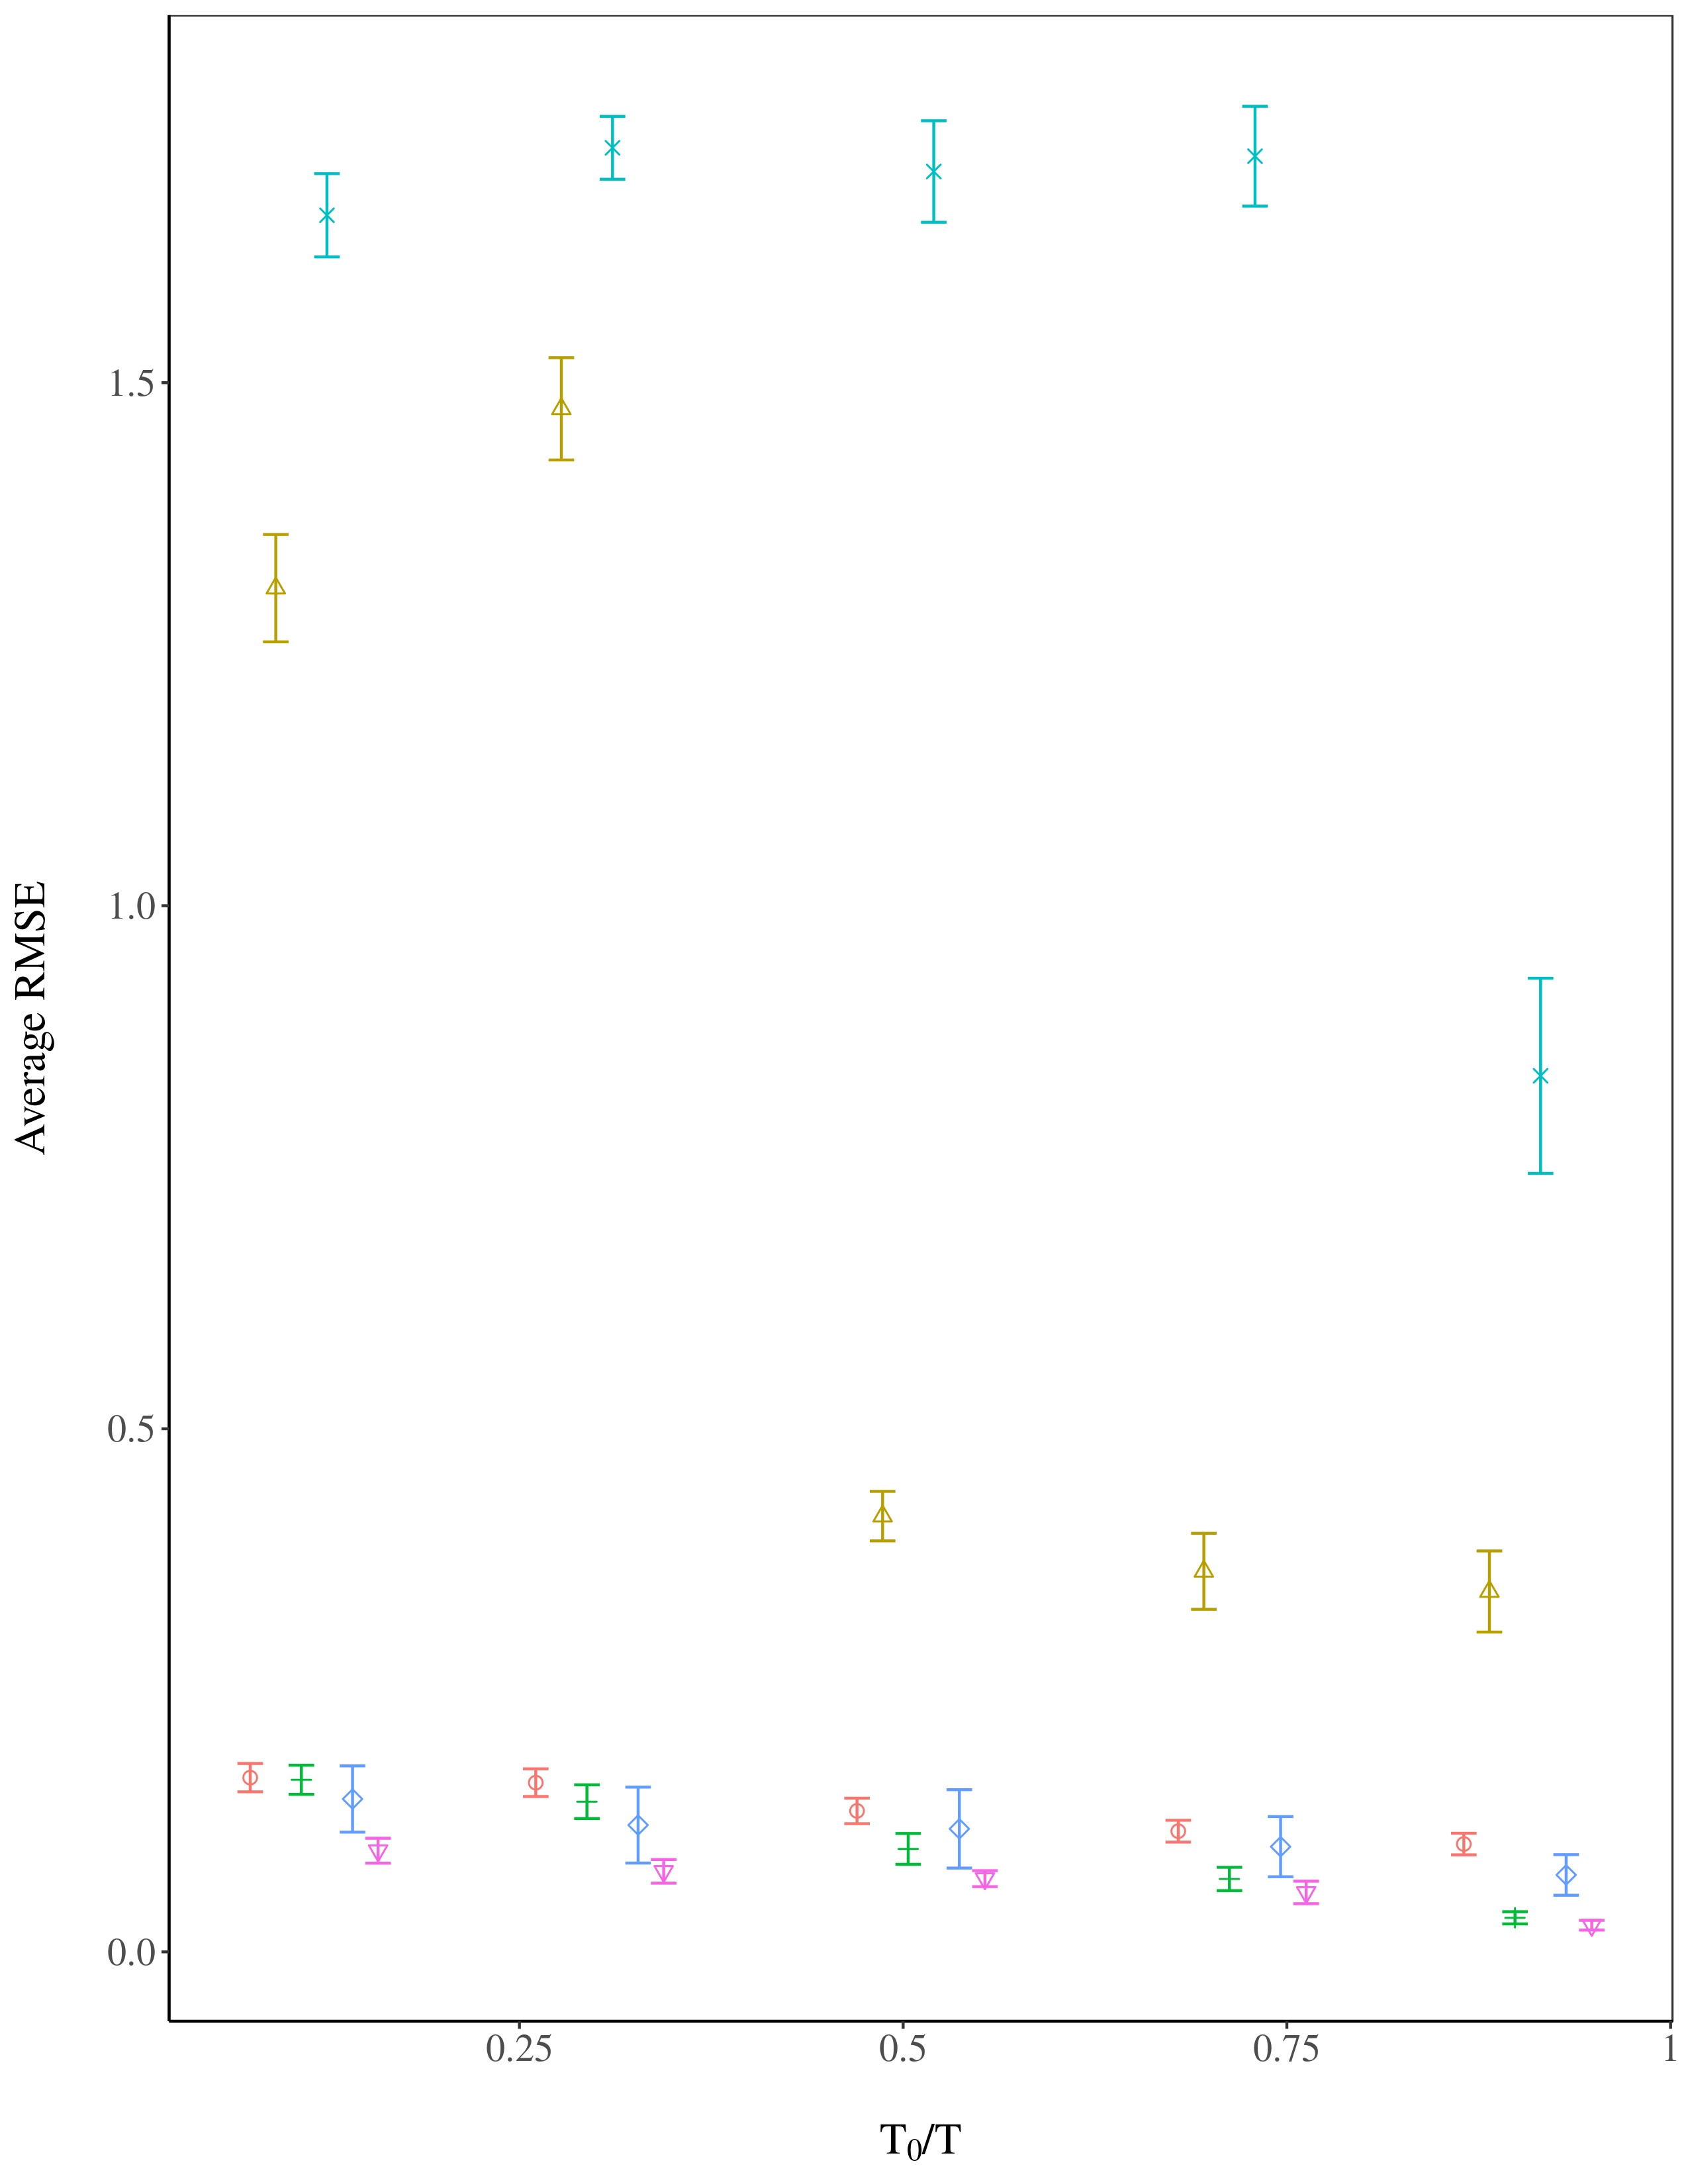
\includegraphics[width=\textwidth]{/media/jason/Dropbox/github/rnns-causal/results/plots/basque-sim.png}
		\caption{Basque Country terrorism data} 
	\end{subfigure}
	~ 
	\begin{subfigure}[t]{0.48\textwidth}
		\centering
		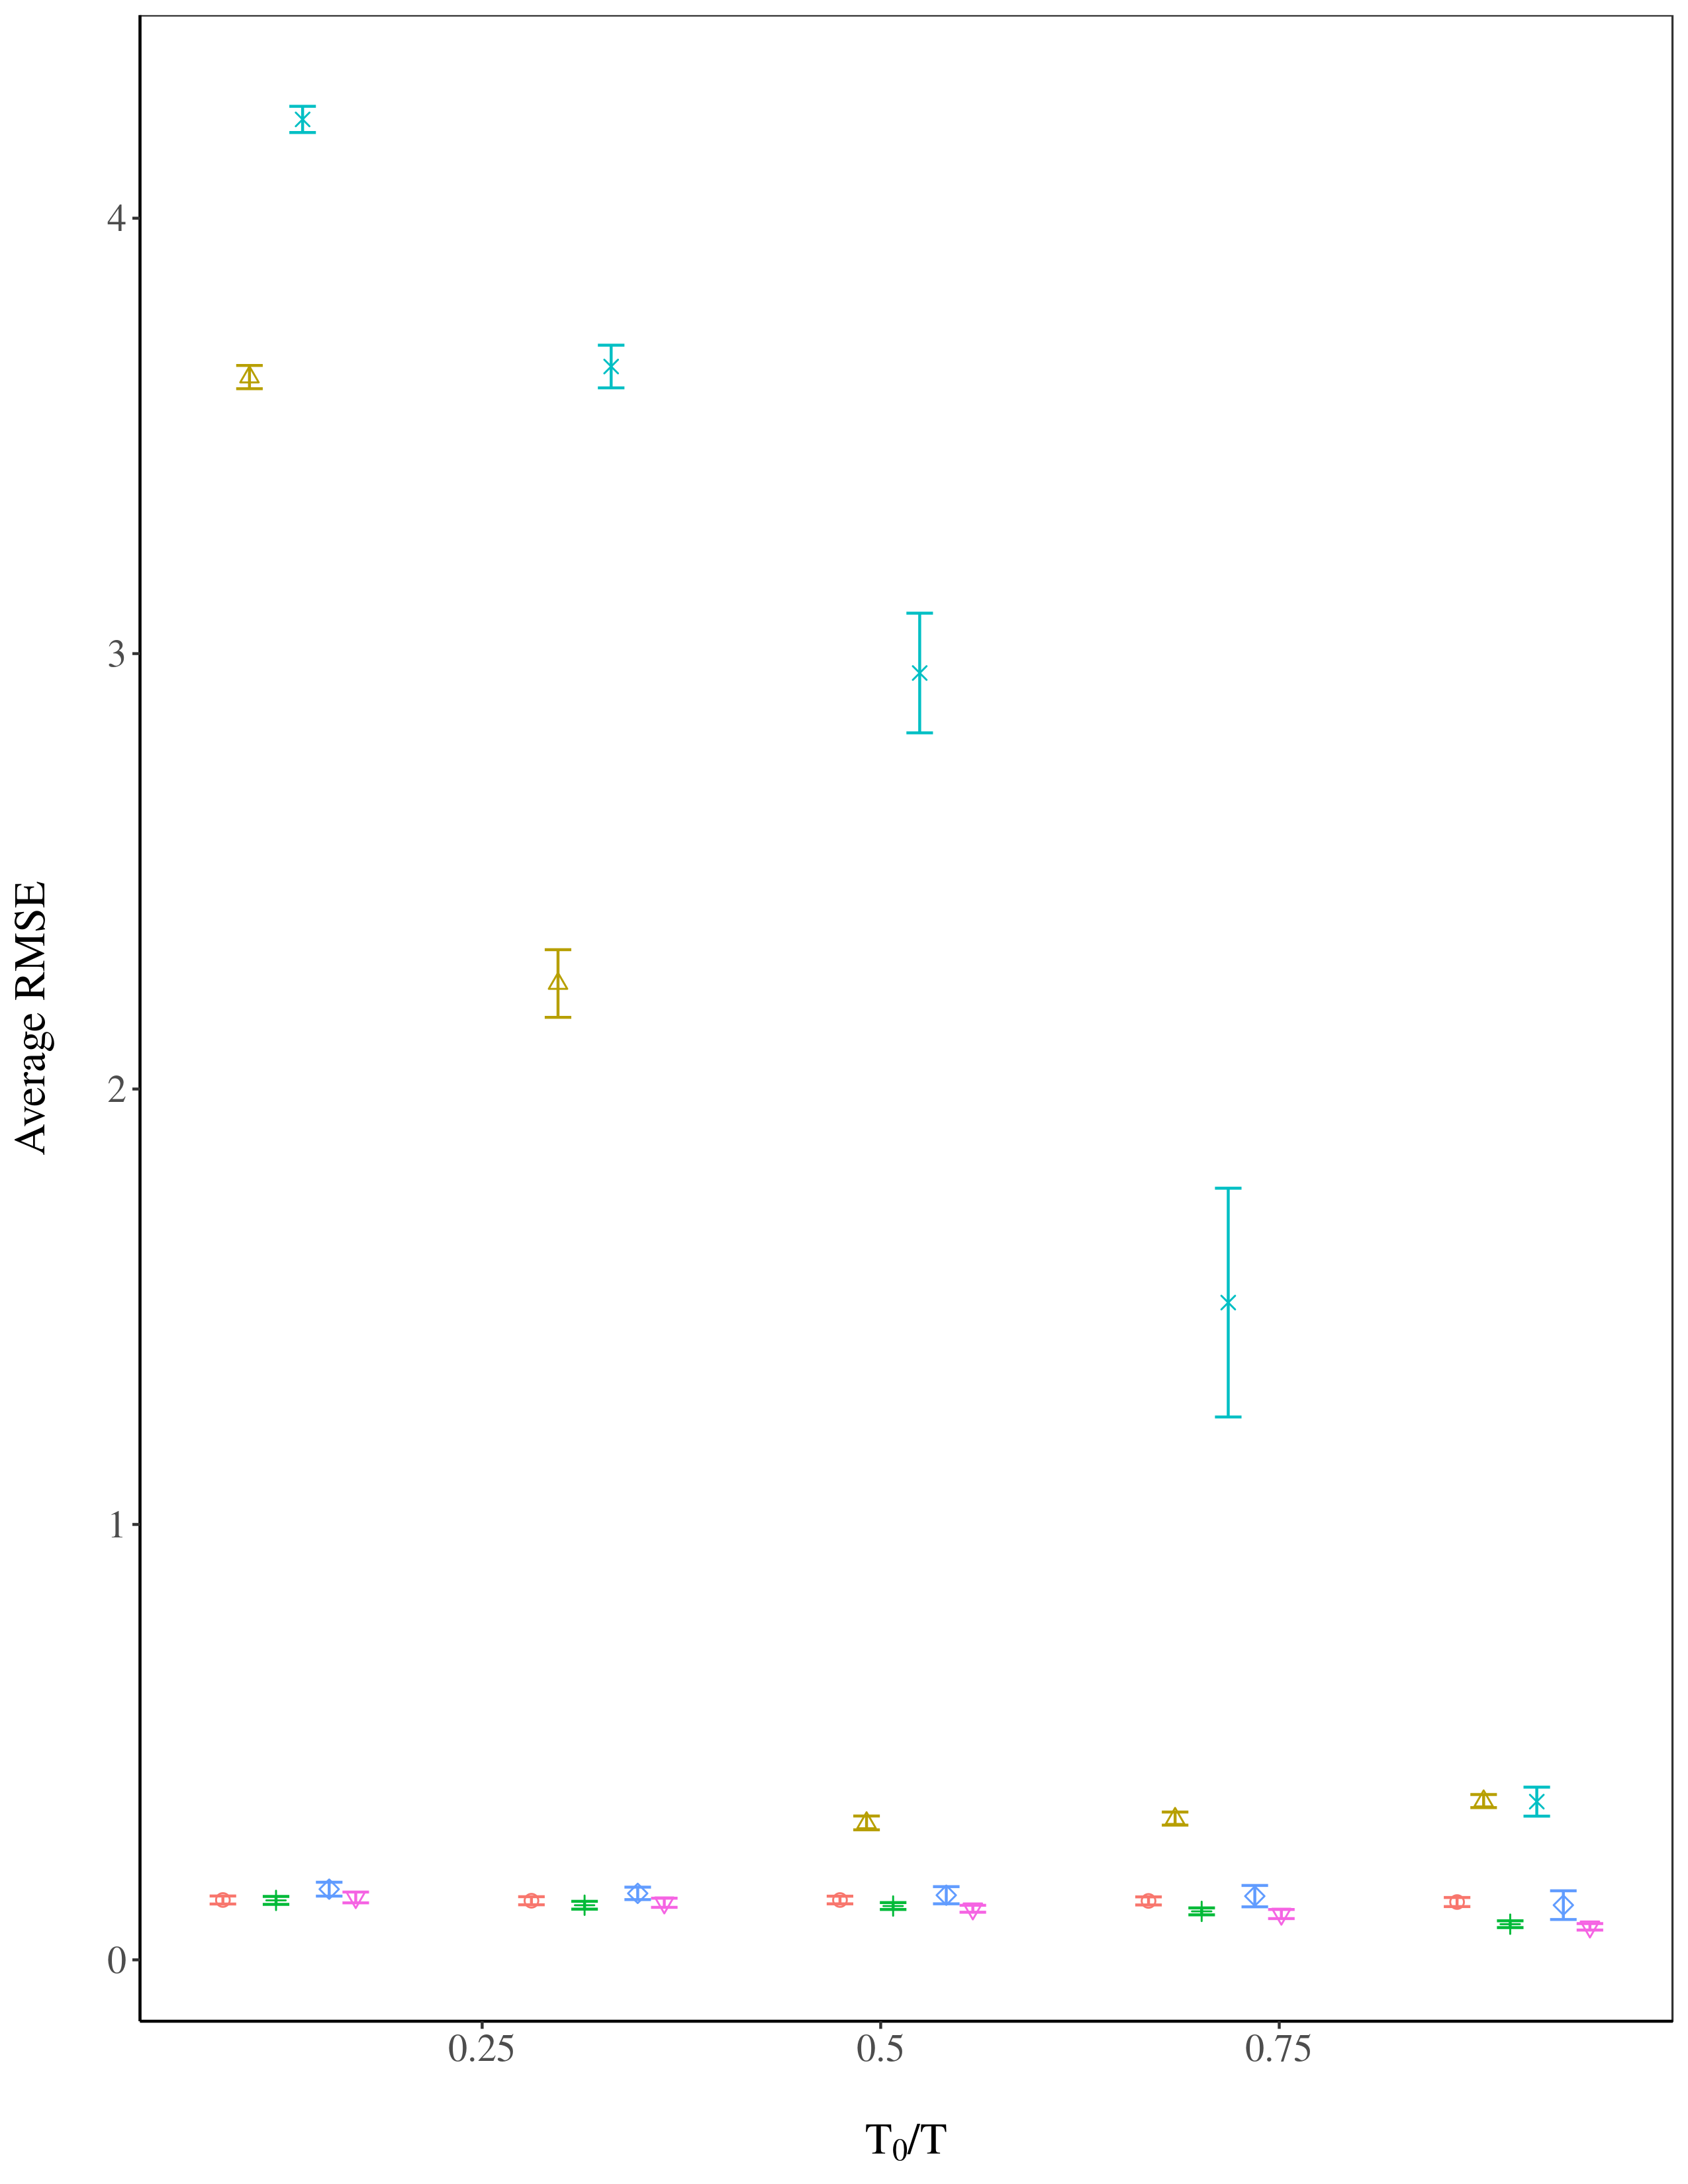
\includegraphics[width=\textwidth]{/media/jason/Dropbox/github/rnns-causal/results/plots/california-sim.png}
		\caption{California smoking ban data} 
	\end{subfigure}
	~ 
	\begin{subfigure}[t]{0.48\textwidth}
		\centering
		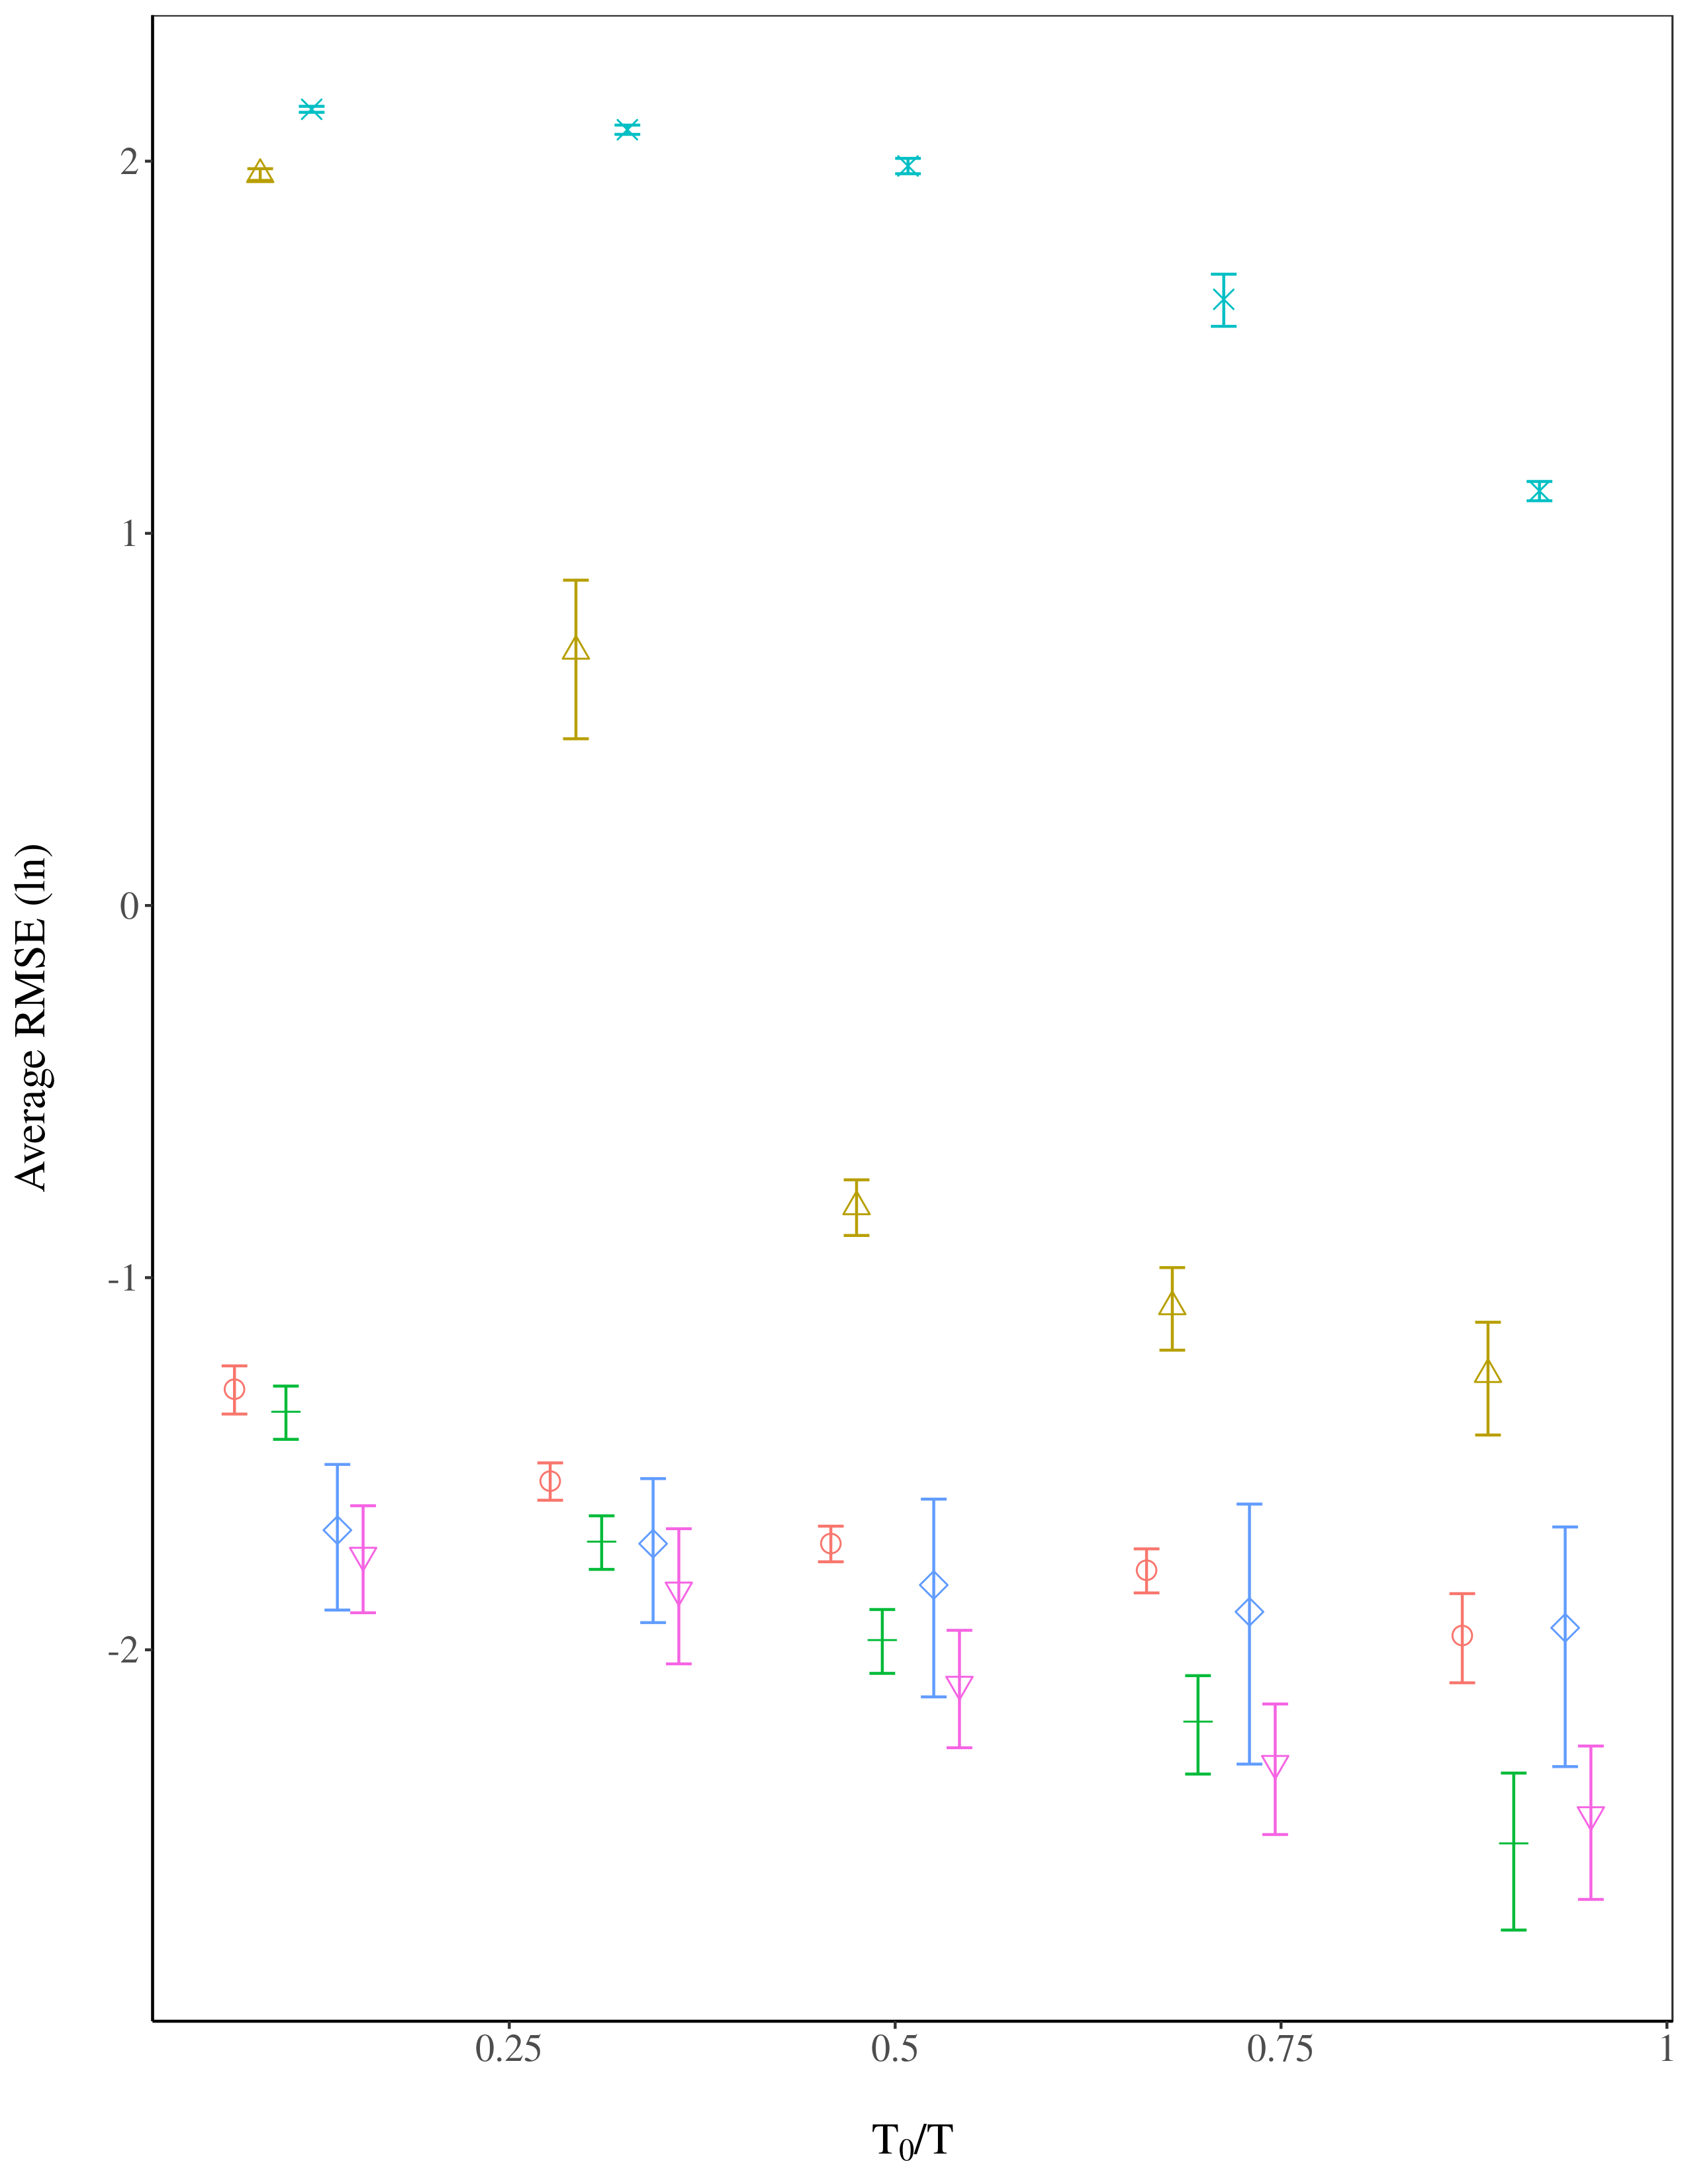
\includegraphics[width=\textwidth]{/media/jason/Dropbox/github/rnns-causal/results/plots/germany-sim.png}
		\caption{West German reunification data}%,
	\end{subfigure}
	\caption{Placebo tests on synthetic control datasets: 
		{\protect\tikz \protect\draw[color={rgb:red,4;green,0;yellow,1}] (0,0) -- plot[mark=o, mark options={scale=2}] (0.25,0) -- (0.5,0);}, DID;
		{\protect\tikz \protect\draw[color={rgb:red,244;green,226;blue,66}] (0,0) -- plot[mark=triangle*, mark options={scale=2,fill=white}] (0.25,0) -- (0.5,0);}, ED; 
		{\protect\tikz \protect\draw[color={rgb:red,0;green,5;blue,1}] (0,0) -- plot[mark=+, mark options={scale=2}] (0.25,0) -- (0.5,0);}, MC-NNM;
		{\protect\tikz \protect\draw[color={rgb:red,66;green,200;blue,244}] (0,0) -- plot[mark=x, mark options={scale=2}] (0.25,0) -- (0.5,0);}, RVAE;
		{\protect\tikz \protect\draw[color={rgb:red,66;green,107;blue,244}] (0,0) -- plot[mark=diamond, mark options={scale=2}] (0.25,0) -- (0.5,0);}, SCM;
		{\protect\tikz \protect\draw[color={rgb:red,244;pink,66;blue,223}] (0,0) -- plot[mark=triangle, mark options={scale=2, rotate=180}] (0.25,0) -- (0.5,0);}, VT-EN.\label{synth-sim}}
\end{figure}

\subsection{Stock market data}

The second battery of placebo tests draws on a dataset of stock market returns compiled by \citet{athey2017matrix}. The dataset consists of daily returns for 2,453 stocks over 3,082 days. In order to track how the error rates vary according to the dimensionality of the data, I create six sub-samples of the first $T$ daily returns of $N$ randomly selected stocks for the pairs $(\text{N}, \text{T}) = (10, 490), (20, 245), (50, 98), (70, 70), (100, 49), (140, 35)$. In each sub-sample, half of the units are randomly selected as treated and $\text{T}_0 = \text{T}/2$.

Figure \ref{stock-sim} reports the average RMSE for each pair with standard errors informed by the error distribution generated by five trial runs. The average RMSE is the lowest for all estimators in the sub-sample $(\text{N}, \text{T}) = (10, 490)$, which reflects the benefit of training on a large number of time periods. Within this sub-sample, encoder-decoder networks and RVAE achieve the lowest average RMSE, followed by MC-NNM, SCM, DID, and lastly, vertical regression. The RNN-based estimators. The RNN-based estimators do comparatively less well when $N \gg T$ since there is not an adequate number of training set pre-periods to learn a good representation. 

\begin{figure}[htbp]
	\centering
	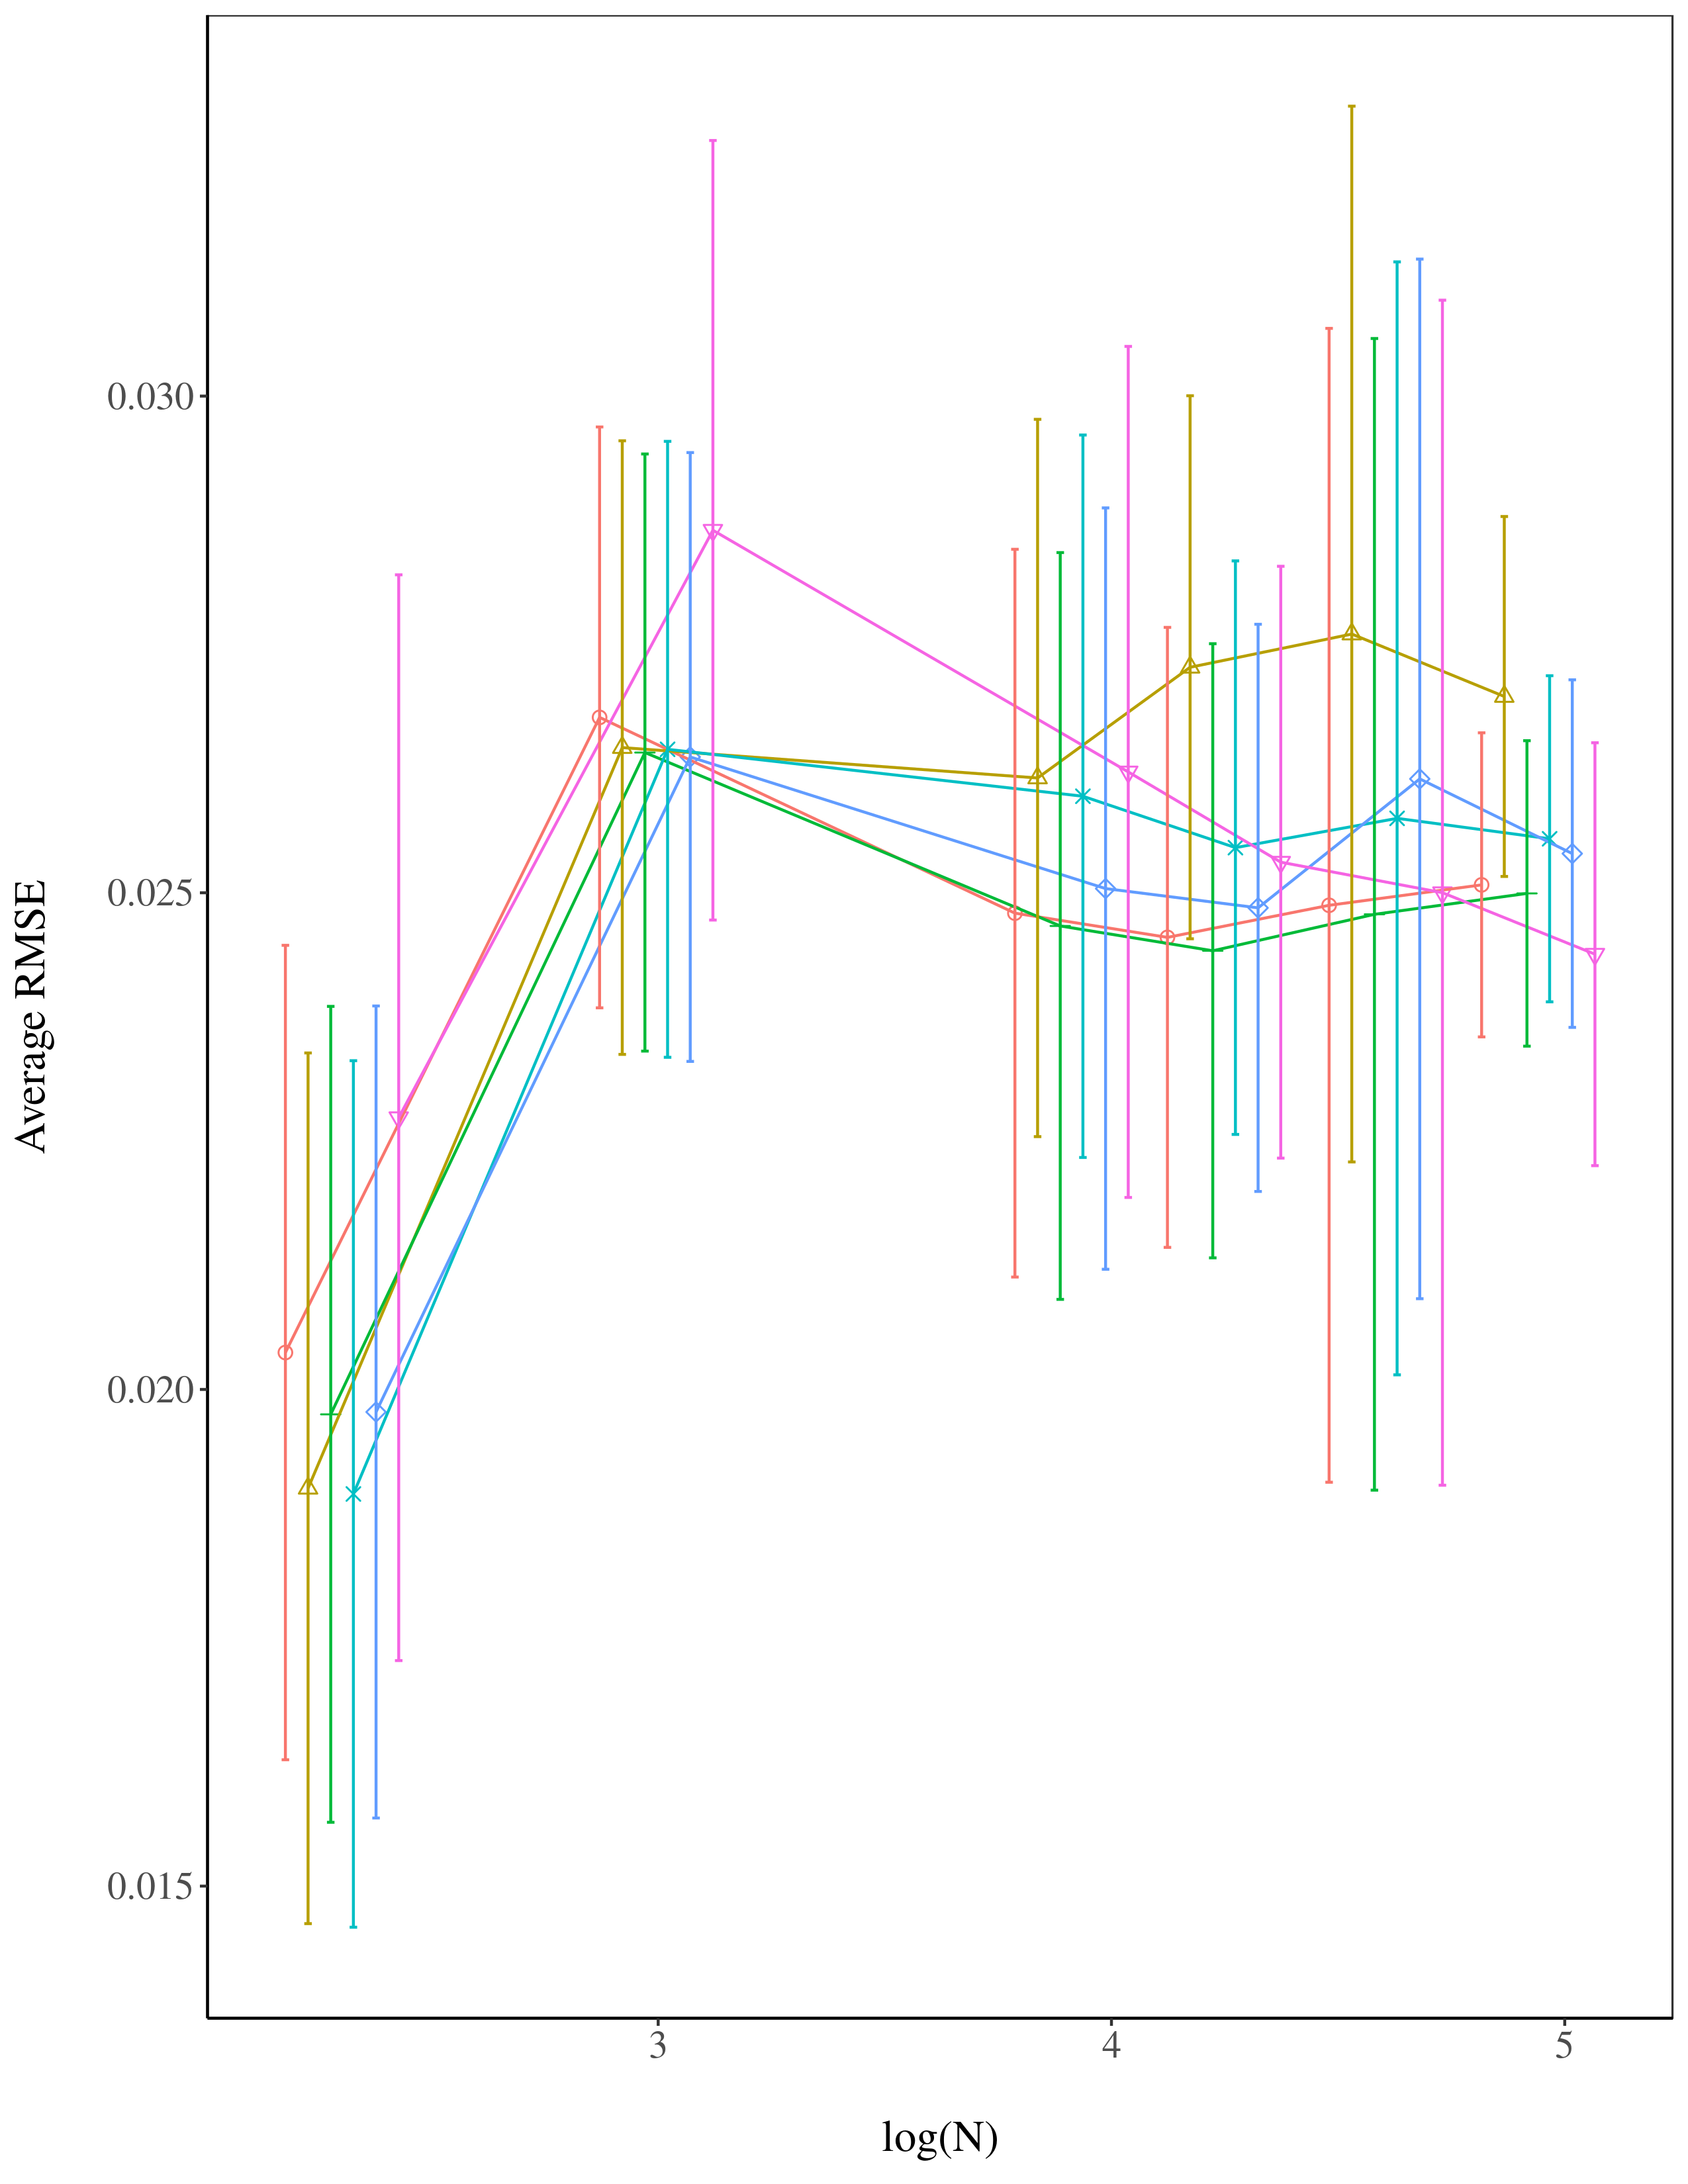
\includegraphics[width=\textwidth]{/media/jason/Dropbox/github/rnns-causal/results/plots/stock-sim.png}
	\caption{Placebo tests on stock market data: 
		{\protect\tikz \protect\draw[color={rgb:red,4;green,0;yellow,1}] (0,0) -- plot[mark=o, mark options={scale=2}] (0.25,0) -- (0.5,0);}, DID;
		{\protect\tikz \protect\draw[color={rgb:red,244;green,226;blue,66}] (0,0) -- plot[mark=triangle*, mark options={scale=2,fill=white}] (0.25,0) -- (0.5,0);}, ED; 
		{\protect\tikz \protect\draw[color={rgb:red,0;green,5;blue,1}] (0,0) -- plot[mark=+, mark options={scale=2}] (0.25,0) -- (0.5,0);}, MC-NNM;
		{\protect\tikz \protect\draw[color={rgb:red,66;green,200;blue,244}] (0,0) -- plot[mark=x, mark options={scale=2}] (0.25,0) -- (0.5,0);}, RVAE;
		{\protect\tikz \protect\draw[color={rgb:red,66;green,107;blue,244}] (0,0) -- plot[mark=diamond, mark options={scale=2}] (0.25,0) -- (0.5,0);}, SCM;
		{\protect\tikz \protect\draw[color={rgb:red,244;pink,66;blue,223}] (0,0) -- plot[mark=triangle, mark options={scale=2, rotate=180}] (0.25,0) -- (0.5,0);}, VT-EN.\label{stock-sim}}
\end{figure}

\section{Hypothesis testing} \label{eval}

In the placebo tests, the counterfactual outcome is known and the estimators can be evaluated in terms of the RMSE between the predicted and actual post-intervention outcomes of placebo treated units. RMSE measures the accuracy of the counterfactual predictions, and consequently the accuracy of the estimated treatment effect. However, this metric does not tell us anything about the statistical significance of estimated treatment effects. 

\citet{abadie2010synthetic} propose a randomization inference approach for calculating the exact distribution of placebo effects under the sharp null hypothesis of no effect. \citet{cavallo2013catastrophic} extends the placebo-based testing approach to the case of multiple (placebo) treated units by constructing a distribution of \emph{average} placebo effects under the null hypothesis. \citet{firpo2018synthetic} derive the conditions under which the randomization inference approach is valid from a finite sample perspective.\footnote{\citet{hahn2017synthetic} analyze the approach from a repeated sampling perspective.} Randomization $p$-values are obtained following these steps:

\begin{enumerate} 
	\item Estimate the observed test static $\upmu^{*}$ by calculating the MSE for all $\text{J}$ control units, which results in a matrix of dimension $(\text{T}-\text{T}_0) \times \text{J}$. Taking the row-wise mean results in a $\text{T}-\text{T}_0$-length array of observed average placebo treated effects. 
	\item Calculate every possible average placebo effect $\upmu$ by randomly sampling without replacement which $\text{J}-1$ control units are assumed to be treated. There are $\mathcal{Q} = \sum\limits_{\text{g}=1}^{\text{J}-1} {\text{J} \choose \text{g}}$ possible average placebo effects. The result is a matrix of dimension $(\text{T}-\text{T}_0) \times \mathcal{Q}$.\footnote{Note that $\mathcal{Q}$ can be computationally burdensome when there are many control units. I set $\mathcal{Q} = 10,000$ in which $\text{J} > 16$.}
	\item Take a column-wise sum of the number of $\upmu$ that are greater than or equal to $\upmu^{*}$.  
\end{enumerate}

Each element of the $(\text{T}-\text{T}_0) \times J$ matrix of counts obtained from the last step is divided by $\mathcal{Q}$ to estimate an array of exact two-sided $p$ values, $\hat{p}$. Assuming that treatment has a constant additive effect $\Delta$, I construct an interval estimate for $\Delta$ by inverting the randomization test. Let $\delta_\Delta$ be the test statistic calculated by subtracting all possible $\mu$ by $\Delta$. I derive a two-sided randomization confidence interval by collecting all values of $\delta_\Delta$ that yield $\hat{p}$ values greater than or equal to a significance level $\alpha$. I find the endpoints of the confidence interval by randomly sampling 500 values of $\Delta$.


\section{Application: Homestead acts and public schooling} \label{schooling-app}

Sociologists and political economists \citep[e.g,][]{meyer1979public,alesina2013nation,bandiera2018nation} have viewed the rapid development of public schooling in the U.S. during the 19th century as a form of nation-building policy. It is argued in this literature that states across the U.S. adopted compulsory primary education means to homogenize the population during the Age of Mass Migration of tens of millions of migrants who arrived to the country between 1850 and 1914. 

An alternative explanation for the rise of public schooling is the view that frontier state governments sought to increase public investments in order to attract eastern migrants following the passage of the Homestead Act (HSA) of 1862, which opened for settlement hundreds of millions of acres of frontier land.  Any adult citizen could apply for a homestead grant of 160 acres of land, provided that they live and make improvements on the land for five years. \citet{engerman2005evolution} argue that the sparse population on the frontier meant that state and local governments competed with each other to attract migrants in order to lower local labor costs and to increase land values and tax revenues. Frontier governments offered migrants broad access to cheap land and property rights, unrestricted voting rights, and a more generous provision of schooling and other public goods.

The HSA may have also increased state schooling expenditures by reducing the degree of land inequality on the frontier. Policies that led to the decentralization of public land are expected to lower land inequality by fixing land grants to 160 acres, thereby encouraging farm sizes to approach their ideal scale. Political economy frameworks \citep[e.g.,][]{acemoglu2008persistence, besley2009origins} emphasize that greater economic power of the ruling class reduces public investments. In the model of \citet{galor2009inequality}, wealthy landowners block education reforms because public schooling favors industrial labor productivity and decreases the value in farm rents. Inequality in this context can be thought of as a proxy for the amount of \emph{de facto} political influence elites have to block reforms.

\subsection{Data and assumptions} \label{educ-data}

I create a state-level measure of state government education spending from the records of 48 state governments during the period of 1783 to 1932 \citep{sylla1993sources} and the records of 16 state governments during the period of 1933 to 1937 \citep{sylla1995sourcesa,sylla1995sourcesb}. Comparable measures for 48 states are drawn from U.S. Census special reports for the years 1902, 1913, 1932, 1942, 1962, 1972, and 1982 \citep{haines2010}.

The data pre-processing steps are as follows. The measure is inflation-adjusted according to the U.S. Consumer Price Index \citep{williamson2017seven} and scaled by the total free population in the decennial census \citep{haines2010}. Missing values are imputed separately in the pre- and -post-periods by carrying the last observation forward and remaining missing values are imputed by carrying the next observation backward. The data are log-transformed to alleviate exponential effects. Lastly, I remove states with no variance in the pre-period outcomes, resulting in a matrix of size $(\text{N} \times \text{T})= (32 \times 156)$. 

In this application, public land states --- i.e., states crafted from the public domain --- serve as treated units (i.e., test set). State land states, which include states of the original 13 colonies, Maine, Tennessee, Texas, Vermont, and West Virginia, were not directly affected by homestead policies and therefore serve as control units (i.e., training set). The RNN-based approach assumes the distribution of $\boldsymbol{X}^{\text{train}}$ and $\boldsymbol{X}^{\text{test}}$ are similar. The assumption may be violated in the application because the state land state governments had already been well-developed by the time of the passage of the homestead laws.

I weight the training loss by  propensity scores in order to minimize distributional discrepancy between the training and test set inputs. The propensity scores are estimated via logistic regression with unit-specific, pre-intervention covariates including state-level average farm sizes measured in the 1860 and average farm values measured in the 1850 and 1860 censuses \citep{haines2010}, which control for homesteaders migrating to more productive land. To control for selection bias arising from differences in access to frontier lands, I create a measure of total miles of operational track per square mile aggregated to the state-level using digitized railroad maps provided by \citet{atack2013use}. 

Fig. \ref{educ-dense} shows that the training and test set input distributions weighted by the propensity scores are visually similar. However, a weighted two-sided t-test rejects the null of equivalence for the difference-in-means between the two distributions ($t= \boldsymbol{\bar{X}}^{\text{train}} - \boldsymbol{\bar{X}}^{\text{test}} = -0.86$; $\sigma_t = 0.07$; $p < 0.01$). While the no interference assumption cannot directly be tested, it is likely that state land states were indirectly affected by the out-migration of homesteaders from frontier states. 

Aggregating to the state level approximately 1.46 million individual land patent records authorized under the HSA, I determine that the earliest homestead entries occurred in 1869 in about half of the frontier states, about seven years following the enactment of the 1862 Homestead Act.\footnote{Land patent records provide information on the initial transfer of land titles from the federal government and are made accessible online by the U.S. General Land Office (\url{https://glorecords.blm.gov}).} Using this information, I set $\text{T}_0 = 87$, which leaves $\text{T} - \text{T}_0 = 69$ time periods when half of the states are exposed to treatment. While the approach assumes that treatment adoption is simultaneous across states, the date of initial treatment exposure varied as new frontier land opened between the period of 1869 to 1902. 

\subsection{Estimates}

Prior to analyzing the data, I conduct placebo tests on the education spending data similar to those described in Section \ref{synth-placebo}. Figure \ref{educ-sim} presents the average RMSE calculated on the control unit outcomes with standard errors originating from 10 runs. In line with the previous placebo tests, the RNN-based estimators yield error rates comparable to the alternative estimators only when there are sufficient pre-period observations to train on; in this case, when $\text{T}_0/\text{T} \geq 0.5$. We can be reasonably confident that the RNN-based estimators will be at least as accurate as the other estimators since $\text{T}_0/\text{T} = 0.55$ in this application. 

Next, I train a encoder-decoder network on the training set of state land states and use the learned weights to predict the counterfactual time-series of public land states.\footnote{Figure \ref{educ-loss} records the evolution of training and validation loss of the networks over 1,000 epochs.} The top panel of Figure \ref{educ-ed} compares the observed time-series of treated units and control units along with the predicted outcomes of treated units. The dashed vertical line represents the first year of treatment exposure in 1869. We are primarily interested in the difference in the observed and predicted treated unit outcomes, which is the quantity $\boldsymbol{\hat{\phi}}$ calculated by (\ref{eq:pointwise}). These per-period causal impacts are plotted in the bottom panel and are bounded by 95\% randomization confidence intervals. 

Counterfactual predictions of state government education spending in the absence of the HSA generally tracks the observed control time-series until the turn of the 19$^\text{th}$ century, at which the counterfactual flattens and diverges from the increasing observed control time-series. This delay can potentially be explained by the fact that homestead entries did not substantially accumulate until after Congress prohibited the sale of public land in 1889 in all states except Missouri \citep{gates1941land,gates1979federal}, as visualized by the per-capita number of homestead entries in each state (Figure \ref{fig:homestead-heatmap}). 

Taking the mean of post-period impacts, I estimate that the impact of the HSA on the state government spending of states exposed to homesteads is 0.69 [-0.19, 2.01]. The confidence intervals surrounding this estimate contains zero, which implies that the estimated impact is not significantly more extreme than the exact distribution of average placebo effects under the null hypothesis. Examining the time-specific causal estimates reveals that fifty years after the first homestead entry, the estimated impact of the HSA on state government education spending in 1919 is 0.68 log points [0.13, 1.24]. The confidence intervals surrounding this time-specific estimate does not contain zero, which implies that the estimated impact is significantly more extreme than the average placebo effects. To put the magnitude of the point estimate in perspective, it represents about 3\% of the total school expenditures per-capita in 1929.\footnote{Data on total school expenditures per-capita of total population are from \citet{snyder2010digest}.}
 
\begin{figure}[htbp]
	\centering
	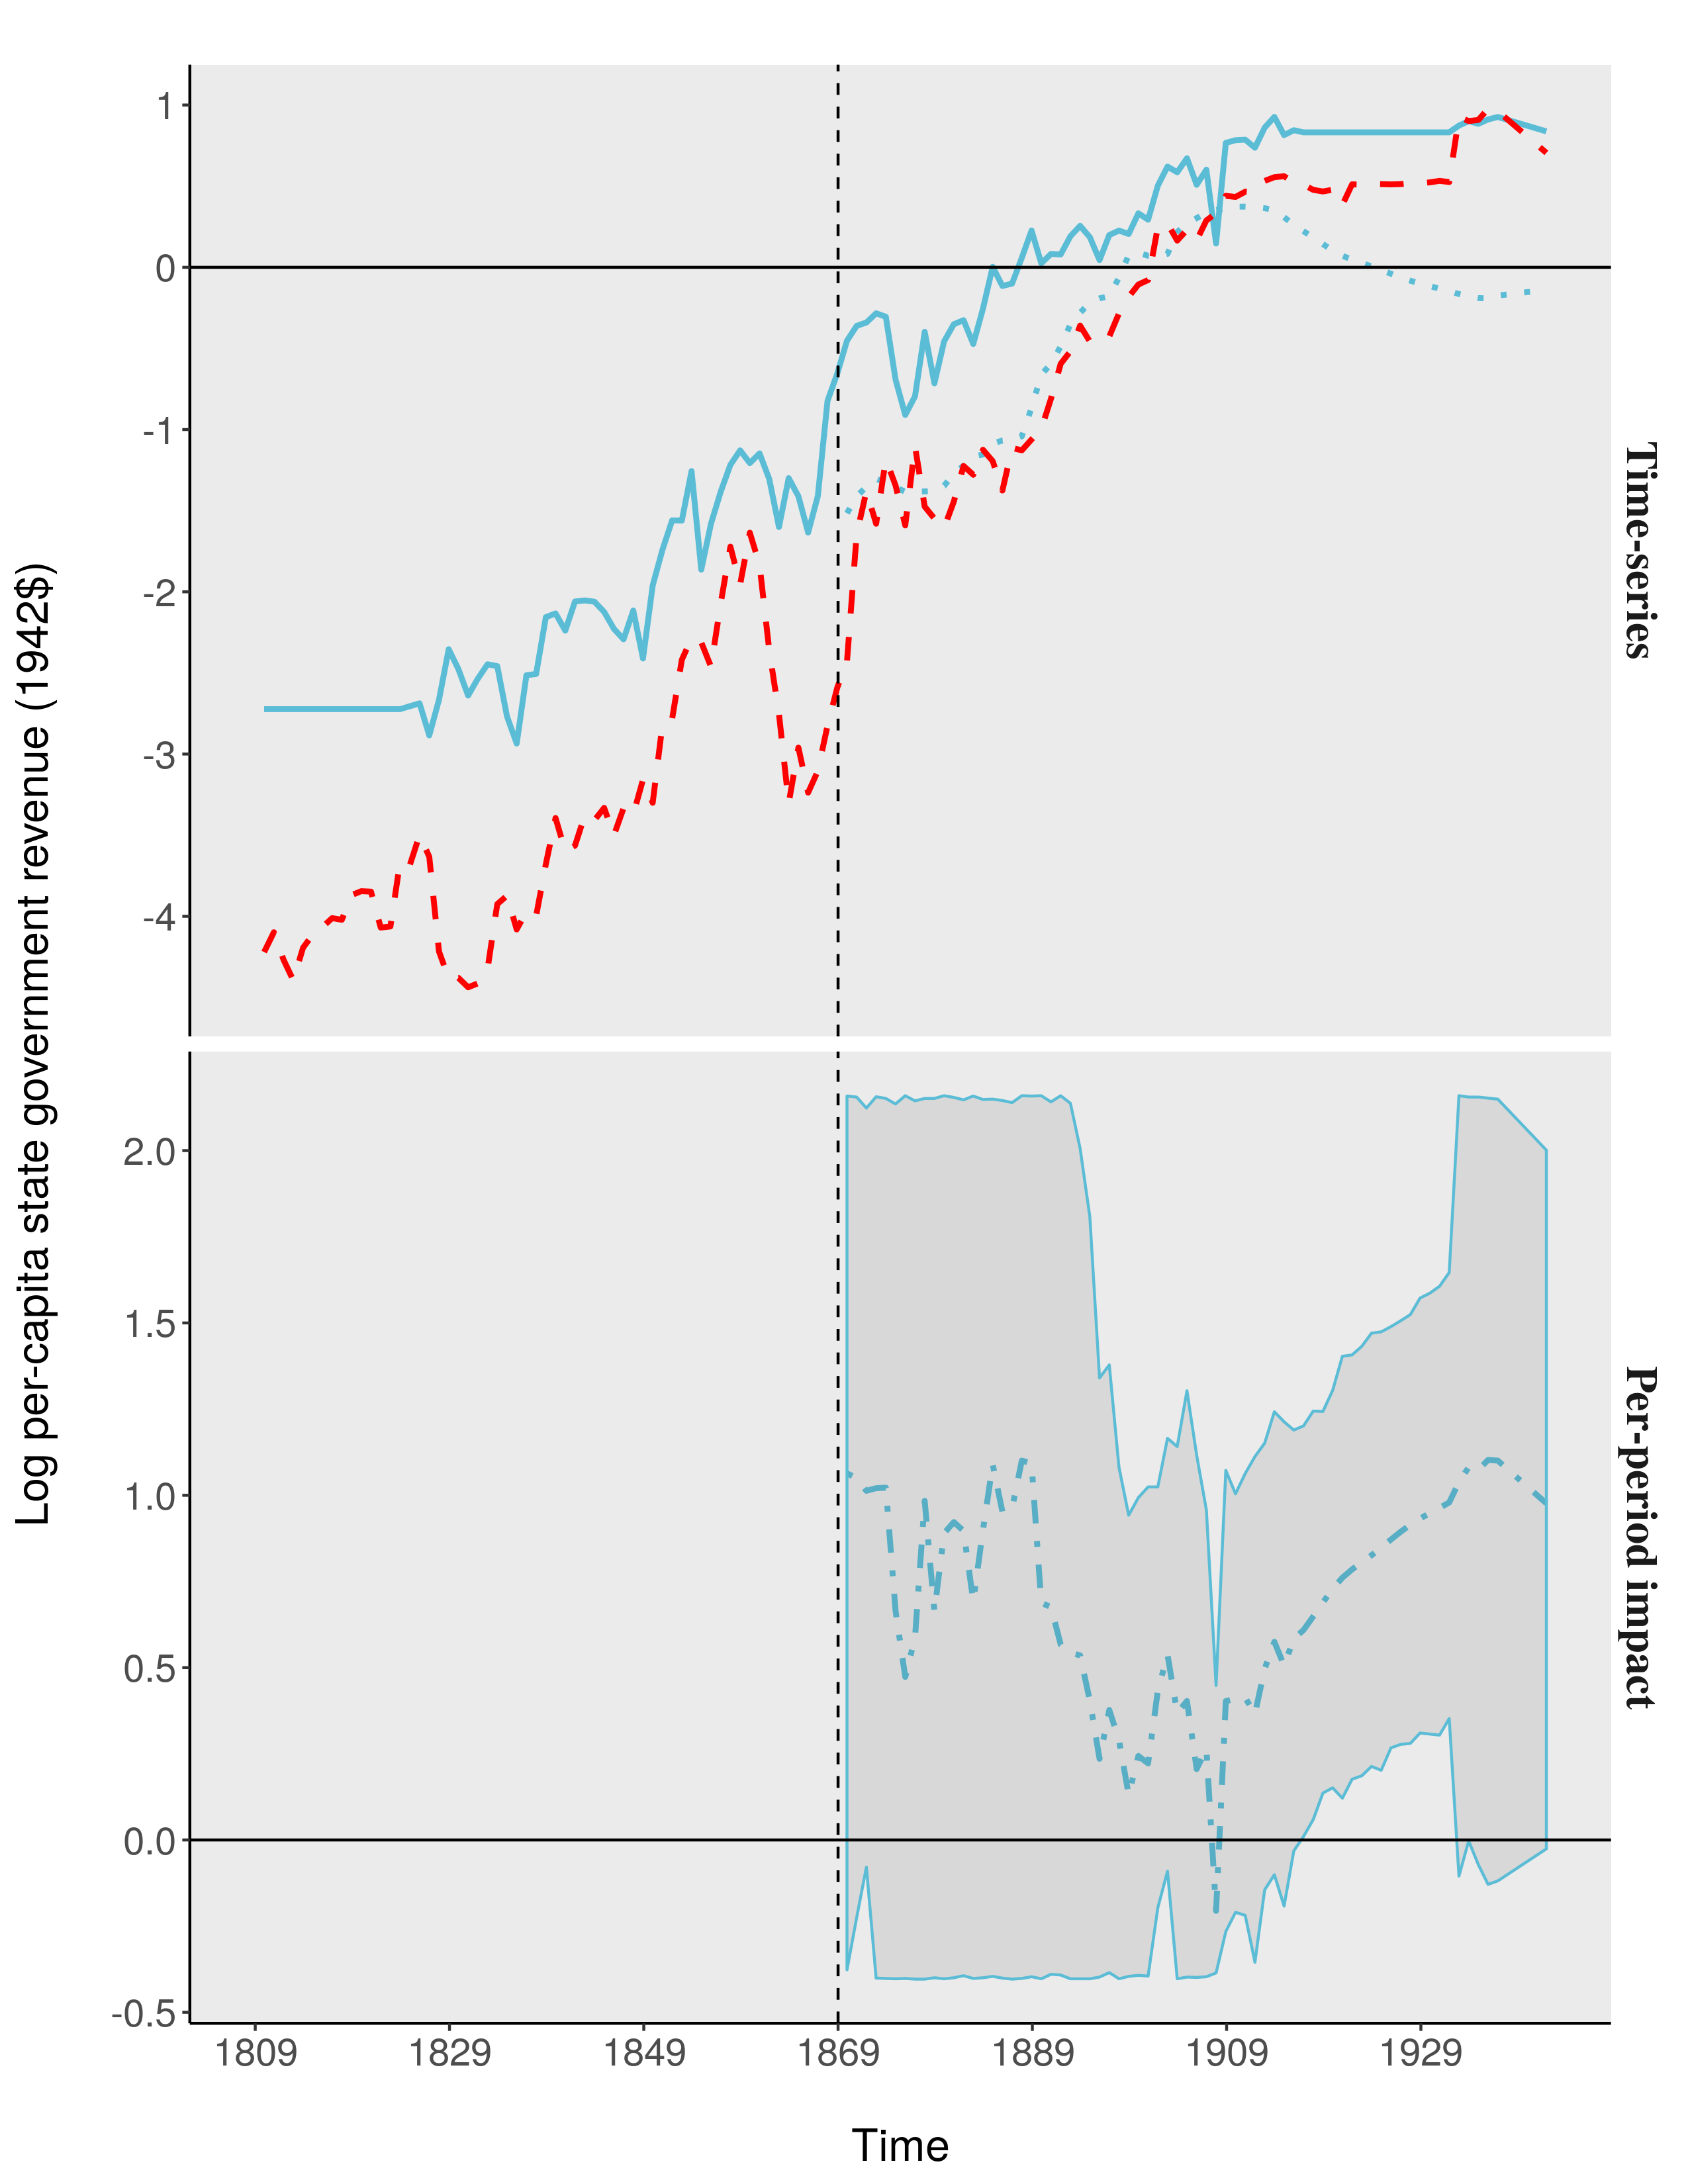
\includegraphics[width=\textwidth]{/media/jason/Dropbox/github/rnns-causal/results/plots/educ-ed.png}
	\caption{Encoder-decoder estimates of the impact of the HSA on state government education spending, 1809 to 1982:		{\color{Darjeeling15}{\sampleline{}}}, observed treated;
		{\color{Darjeeling11}{\sampleline{dashed}}}, observed control;
		{\color{Darjeeling15}{\sampleline{dotted}}}, counterfactual treated;
		{\color{Darjeeling15}{\sampleline{dash pattern=on .7em off .2em on .05em off .2em}}}, $\boldsymbol{\hat{\phi}}$.\label{educ-ed}} 
\end{figure}

\section{Conclusion} \label{conclusion}

This paper makes a methodological contribution in proposing a novel alternative to the SCM for estimating the effect of a policy intervention on an outcome over time in settings where appropriate control units are unavailable. The SCM is growing in popularity in the social sciences despite its limitations --- the most obvious being that the choice of specification can lead to different results, and thus facilitate $p$-hacking. By inputting only control unit outcomes and not relying on pre-period covariates, the proposed method offers a more principled approach than the SCM. 

The RNN-based approach joins a new generation of data-driven machine learning techniques for generating counterfactual predictions. Machine learning techniques in general have an advantage over the SCM in that they automatically choose appropriate predictors without relying on pretreatment covariates; this capability limits ``researcher degrees of freedom'' that arises from choices on how to specify the model. 

The advantages of RNN-based estimators are numerous. RNNs have an advantage over alternative estimators because they do not assume a specific functional distribution, are specifically structured to exploit temporal dependencies in panel data. RNNs are also capable of handling multiple treated units and can learn nonconvex combinations of control units, which is useful because the model can share parameters across treated units, and thus generate more precise predictions in settings in which treated units share similar data-generating processes.

% summarize placebo tests
%combine mc & rnns approach - multidirectional RNNs 

% assumption of equivalence between input distributions
%alt. approach, like machine translation: training set (XC, XT); test set (YC))

Future research might investigate through simulations how the interaction between RNN complexity (as determined by the number of hidden layers or nodes) and data dimensionality impacts predictive accuracy. Simulations will also allow us to assess the exact impact of data dimensionality, the proportion of treated units, convexity versus non-convexity in the modeled relationship, and the length of the pre-period on the choice between RNNs and the SCM. Future work might formalize a set of assumptions necessary for the RNN-based approach to be valid and provide further proof of consistency of the estimator under these assumptions.

\newpage

\bibliographystyle{rss}
\begin{singlespace}
	\begin{footnotesize}
		\begin{multicols}{2}
			\bibliography{references}
		\end{multicols}
	\end{footnotesize}
\end{singlespace}

\newpage

\begin{appendices}

\setcounter{figure}{0}
\renewcommand{\thefigure}{A\arabic{figure}}
	
\begin{figure}[htbp]
		\centering
		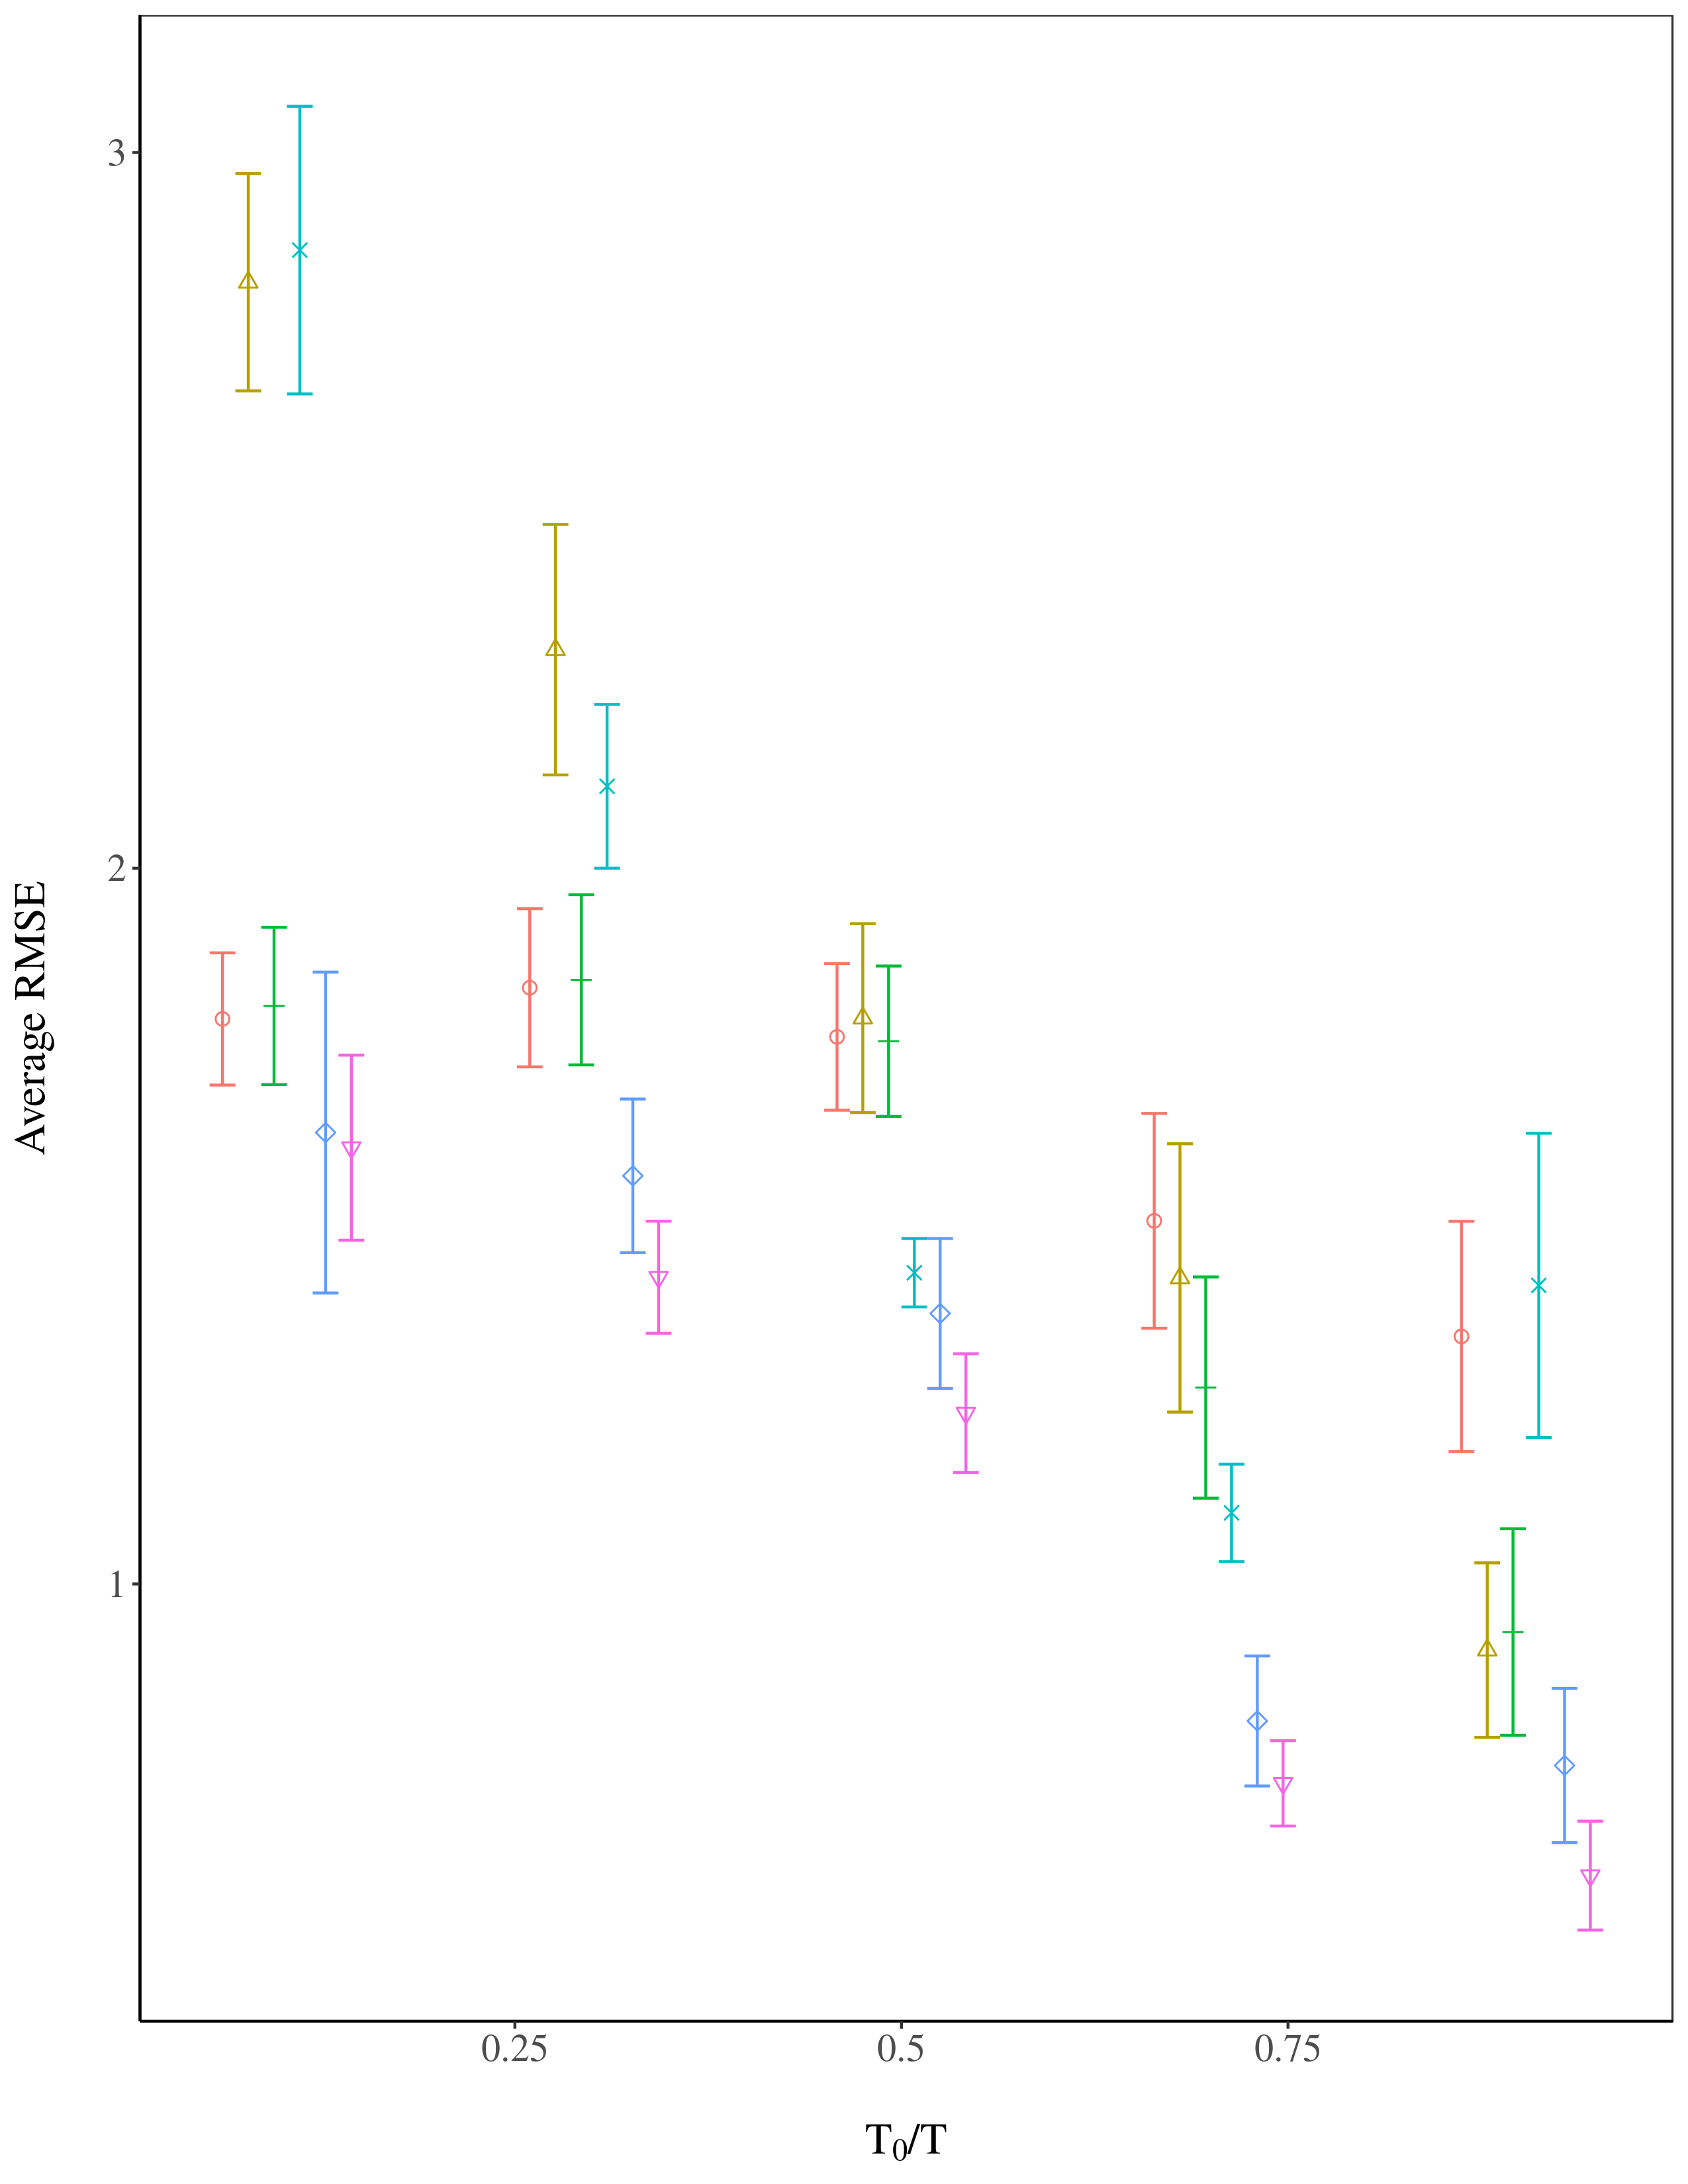
\includegraphics[width=0.9\textwidth]{/media/jason/Dropbox/github/rnns-causal/results/plots/educ-sim.png}
		\caption{Placebo tests on education spending data: 		{\protect\tikz \protect\draw[color={rgb:red,4;green,0;yellow,1}] (0,0) -- plot[mark=o, mark options={scale=2}] (0.25,0) -- (0.5,0);}, DID;
			{\protect\tikz \protect\draw[color={rgb:red,244;green,226;blue,66}] (0,0) -- plot[mark=triangle*, mark options={scale=2,fill=white}] (0.25,0) -- (0.5,0);}, ED; 
			{\protect\tikz \protect\draw[color={rgb:red,0;green,5;blue,1}] (0,0) -- plot[mark=+, mark options={scale=2}] (0.25,0) -- (0.5,0);}, MC-NNM;
			{\protect\tikz \protect\draw[color={rgb:red,66;green,200;blue,244}] (0,0) -- plot[mark=x, mark options={scale=2}] (0.25,0) -- (0.5,0);}, RVAE;
			{\protect\tikz \protect\draw[color={rgb:red,66;green,107;blue,244}] (0,0) -- plot[mark=diamond, mark options={scale=2}] (0.25,0) -- (0.5,0);}, SCM;
			{\protect\tikz \protect\draw[color={rgb:red,244;pink,66;blue,223}] (0,0) -- plot[mark=triangle, mark options={scale=2, rotate=180}] (0.25,0) -- (0.5,0);}, VT-EN.
			\label{educ-sim}}
\end{figure}
	
\begin{figure*}[htbp]
	\centering
	\begin{subfigure}[t]{0.45\textwidth}
		\centering
		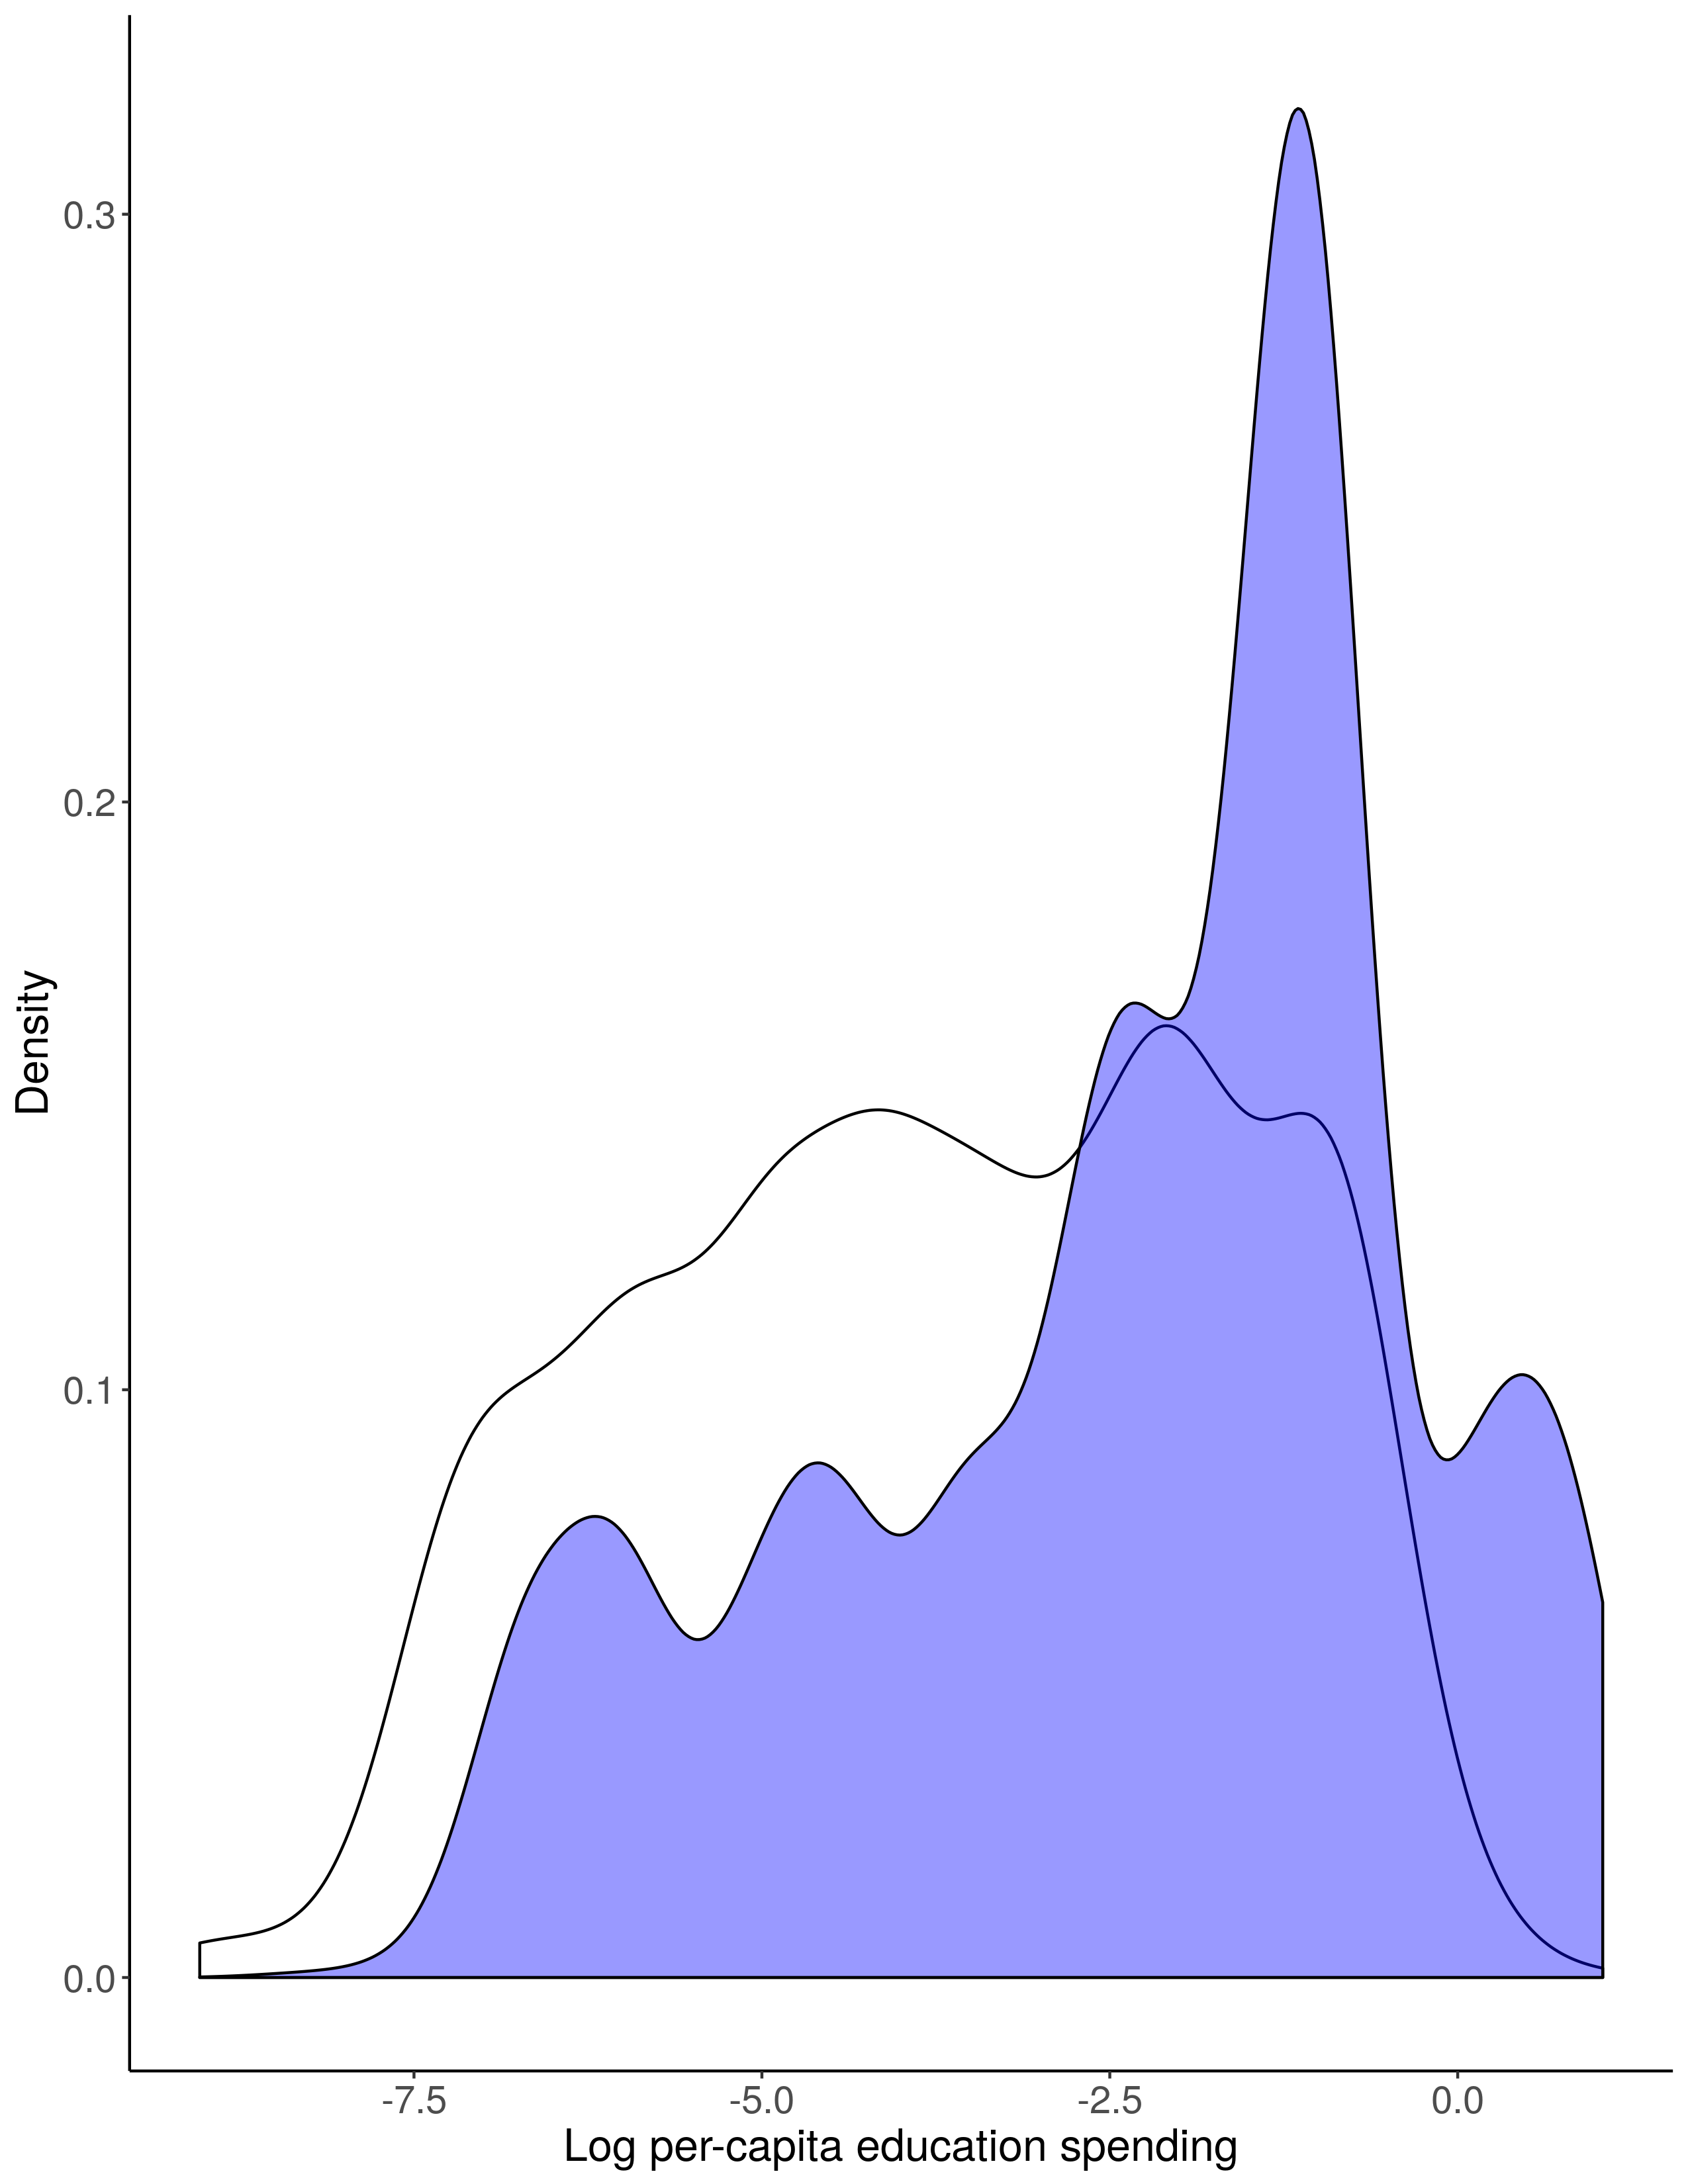
\includegraphics[width=\textwidth]{/media/jason/Dropbox/github/rnns-causal/results/plots/educ-dens.png}
		\caption{Unweighted} 
	\end{subfigure}
	~ 
	\begin{subfigure}[t]{0.45\textwidth}
		\centering
		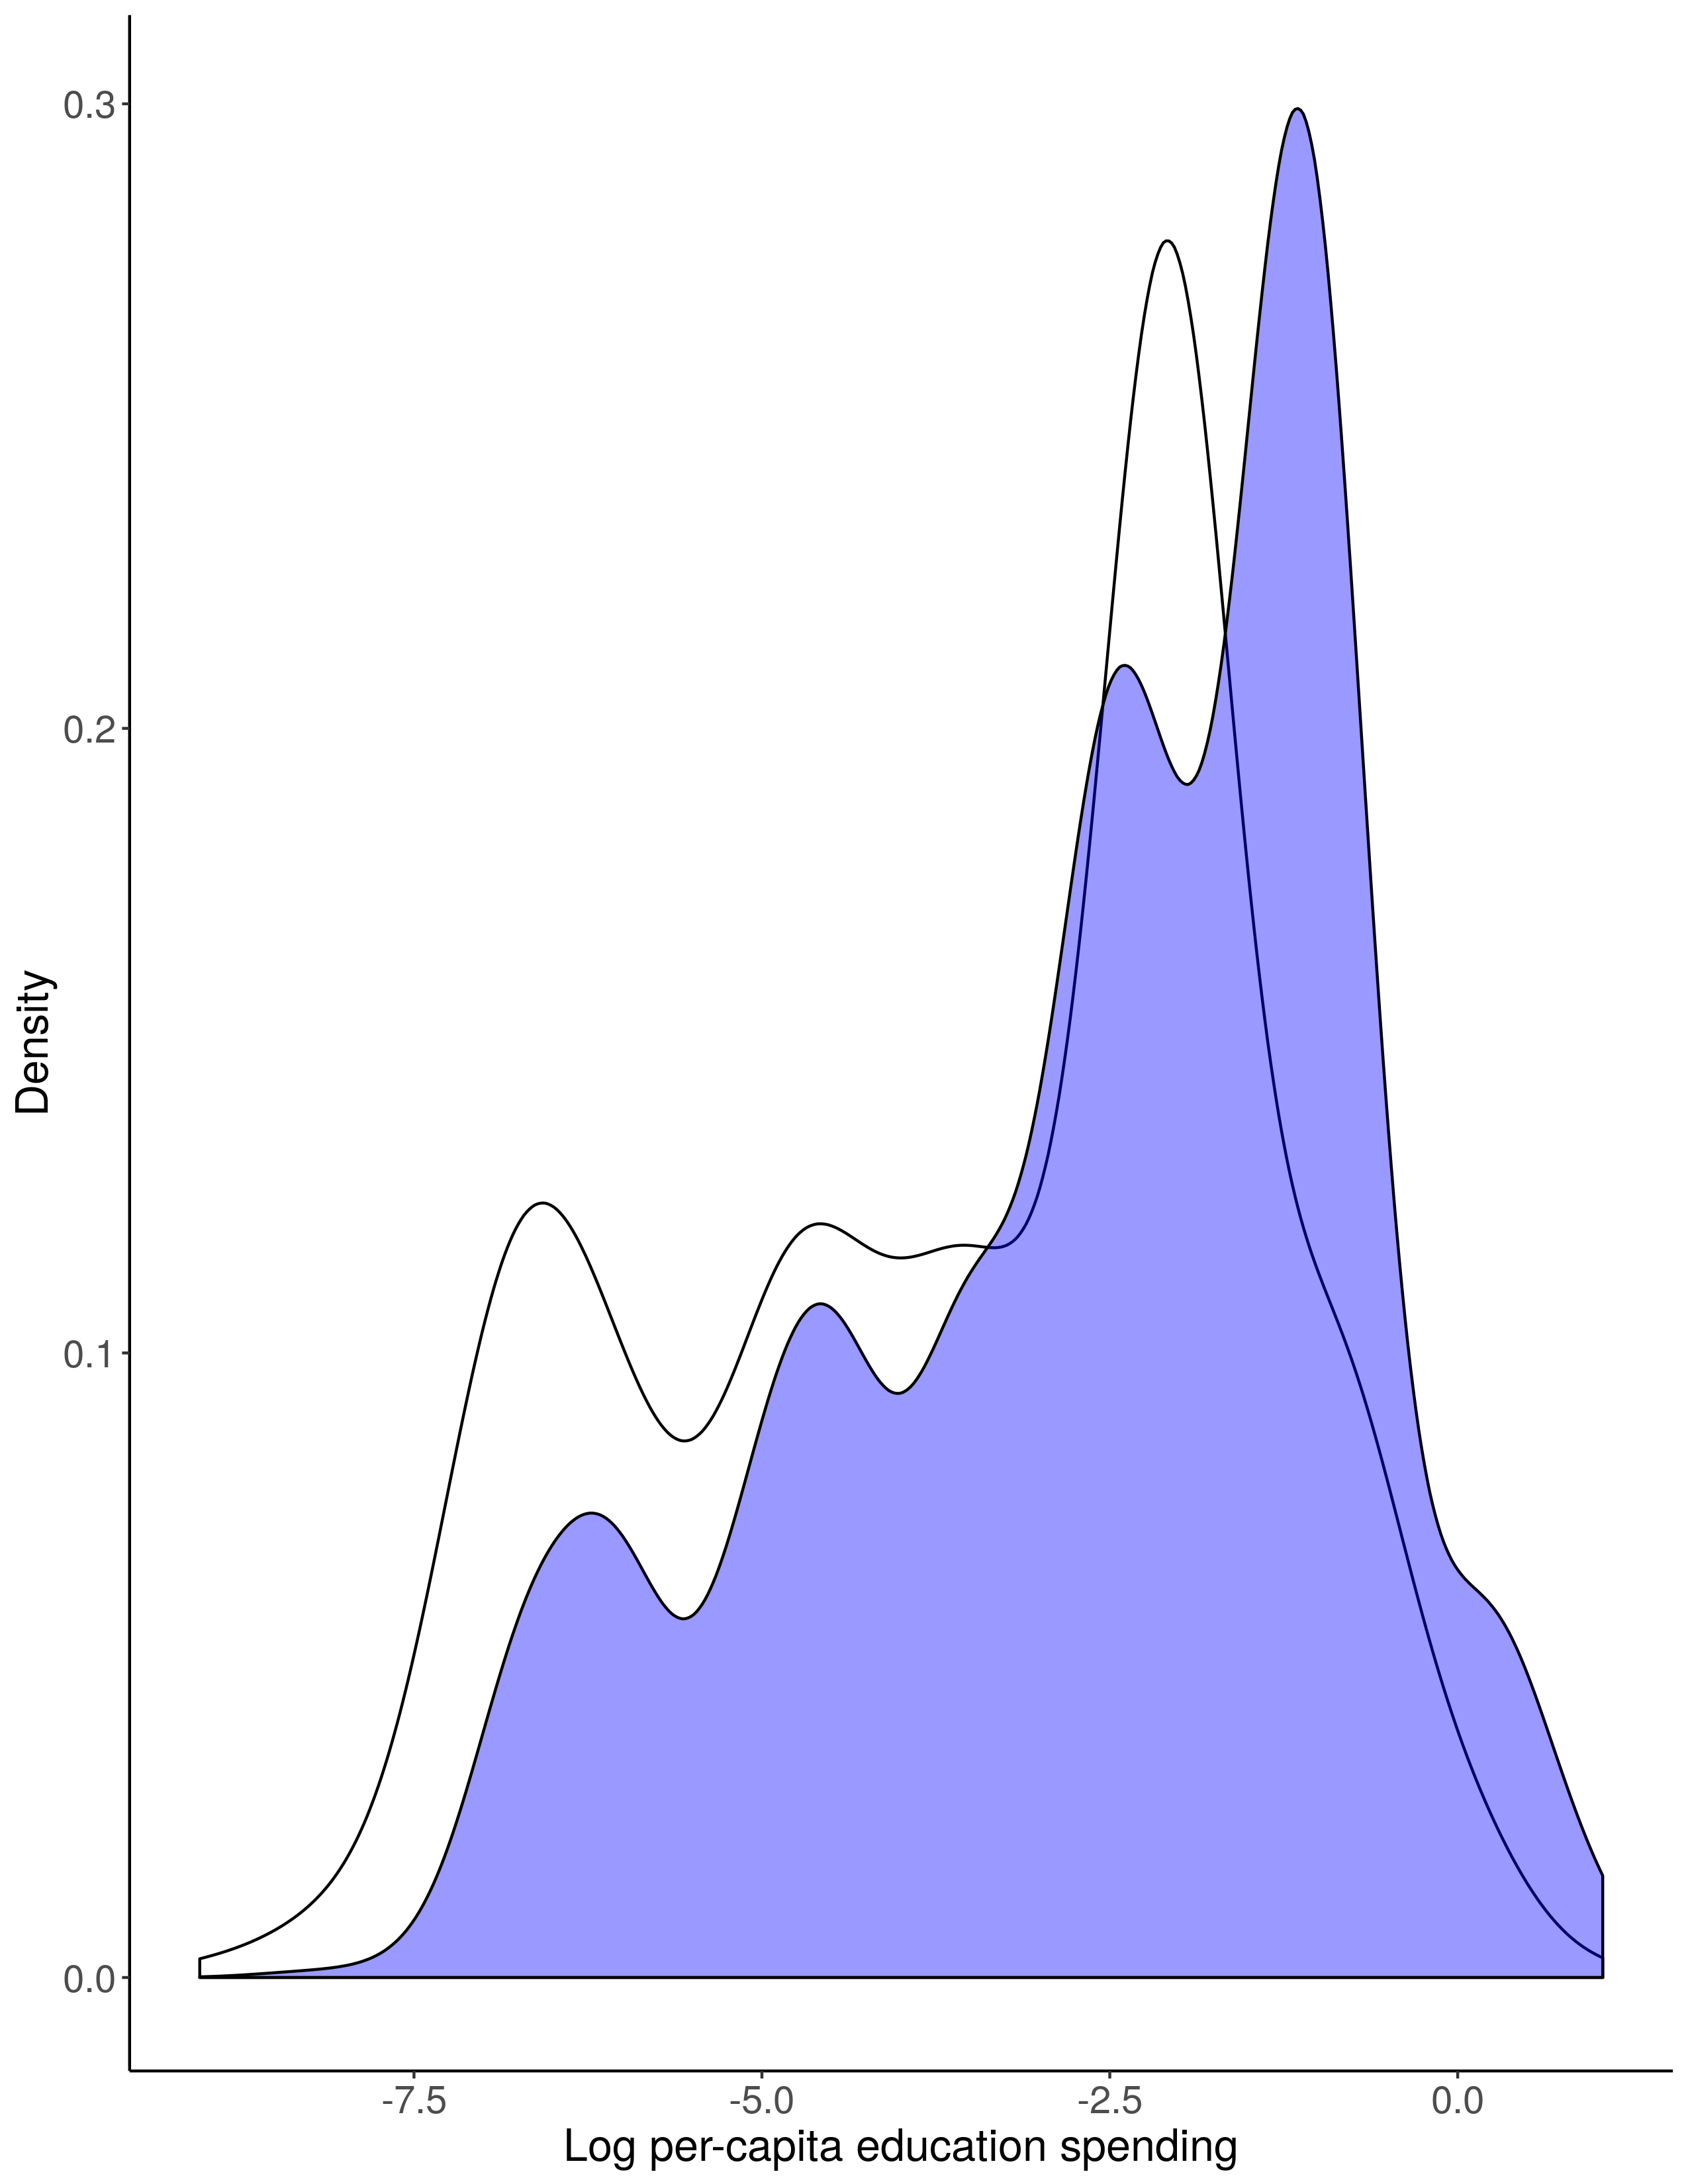
\includegraphics[width=\textwidth]{/media/jason/Dropbox/github/rnns-causal/results/plots/educ-dens-w.png}
		\caption{Weighted\label{educ-dense-w}}
	\end{subfigure}
	\caption{Pre-period densities of log per-capita state government education spending by treatment status. Density in Figure \ref{educ-dense-w} weighted by propensity score. \label{educ-dense}} 
\end{figure*}

\begin{figure}[htbp]
	\centering
	\begin{subfigure}[t]{1\textwidth}
		\centering
		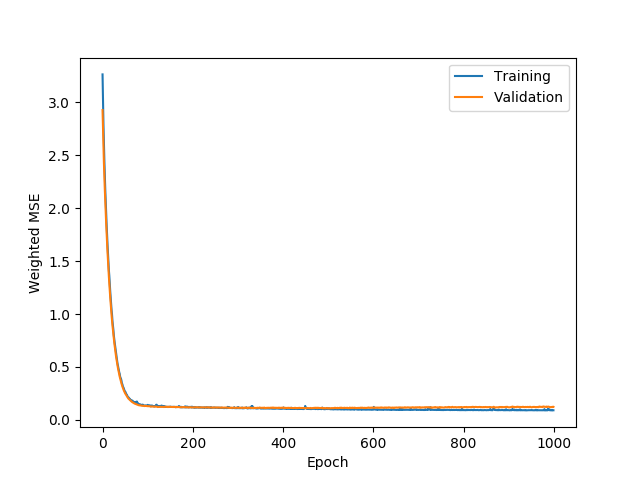
\includegraphics[width=\textwidth]{/media/jason/Dropbox/github/rnns-causal/results/plots/educ-ed-loss.png}
	%	\caption{Encoder-decoder networks} 
	\end{subfigure}
%	~ 
%	\begin{subfigure}[t]{0.8\textwidth}
%		\centering
%		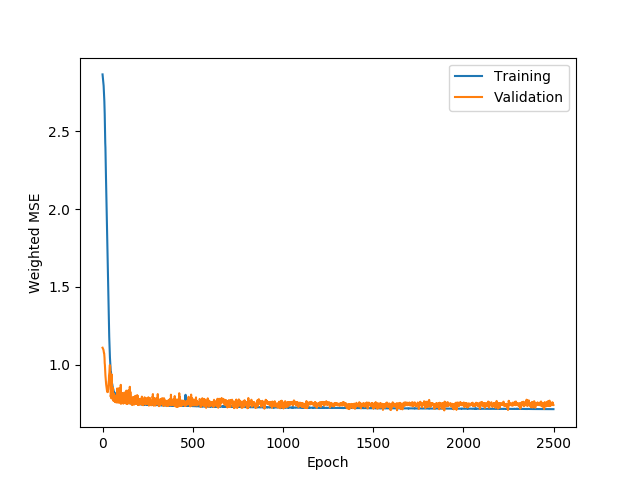
\includegraphics[width=\textwidth]{/media/jason/Dropbox/github/rnns-causal/results/plots/educ-rvae-loss.png}
%		\caption{RVAE}
%	\end{subfigure}
	\caption{Encoder-decoder networks training and validation loss on education spending data. \label{educ-loss}} 
\end{figure}

%\begin{figure}[htbp]
%	\centering
%		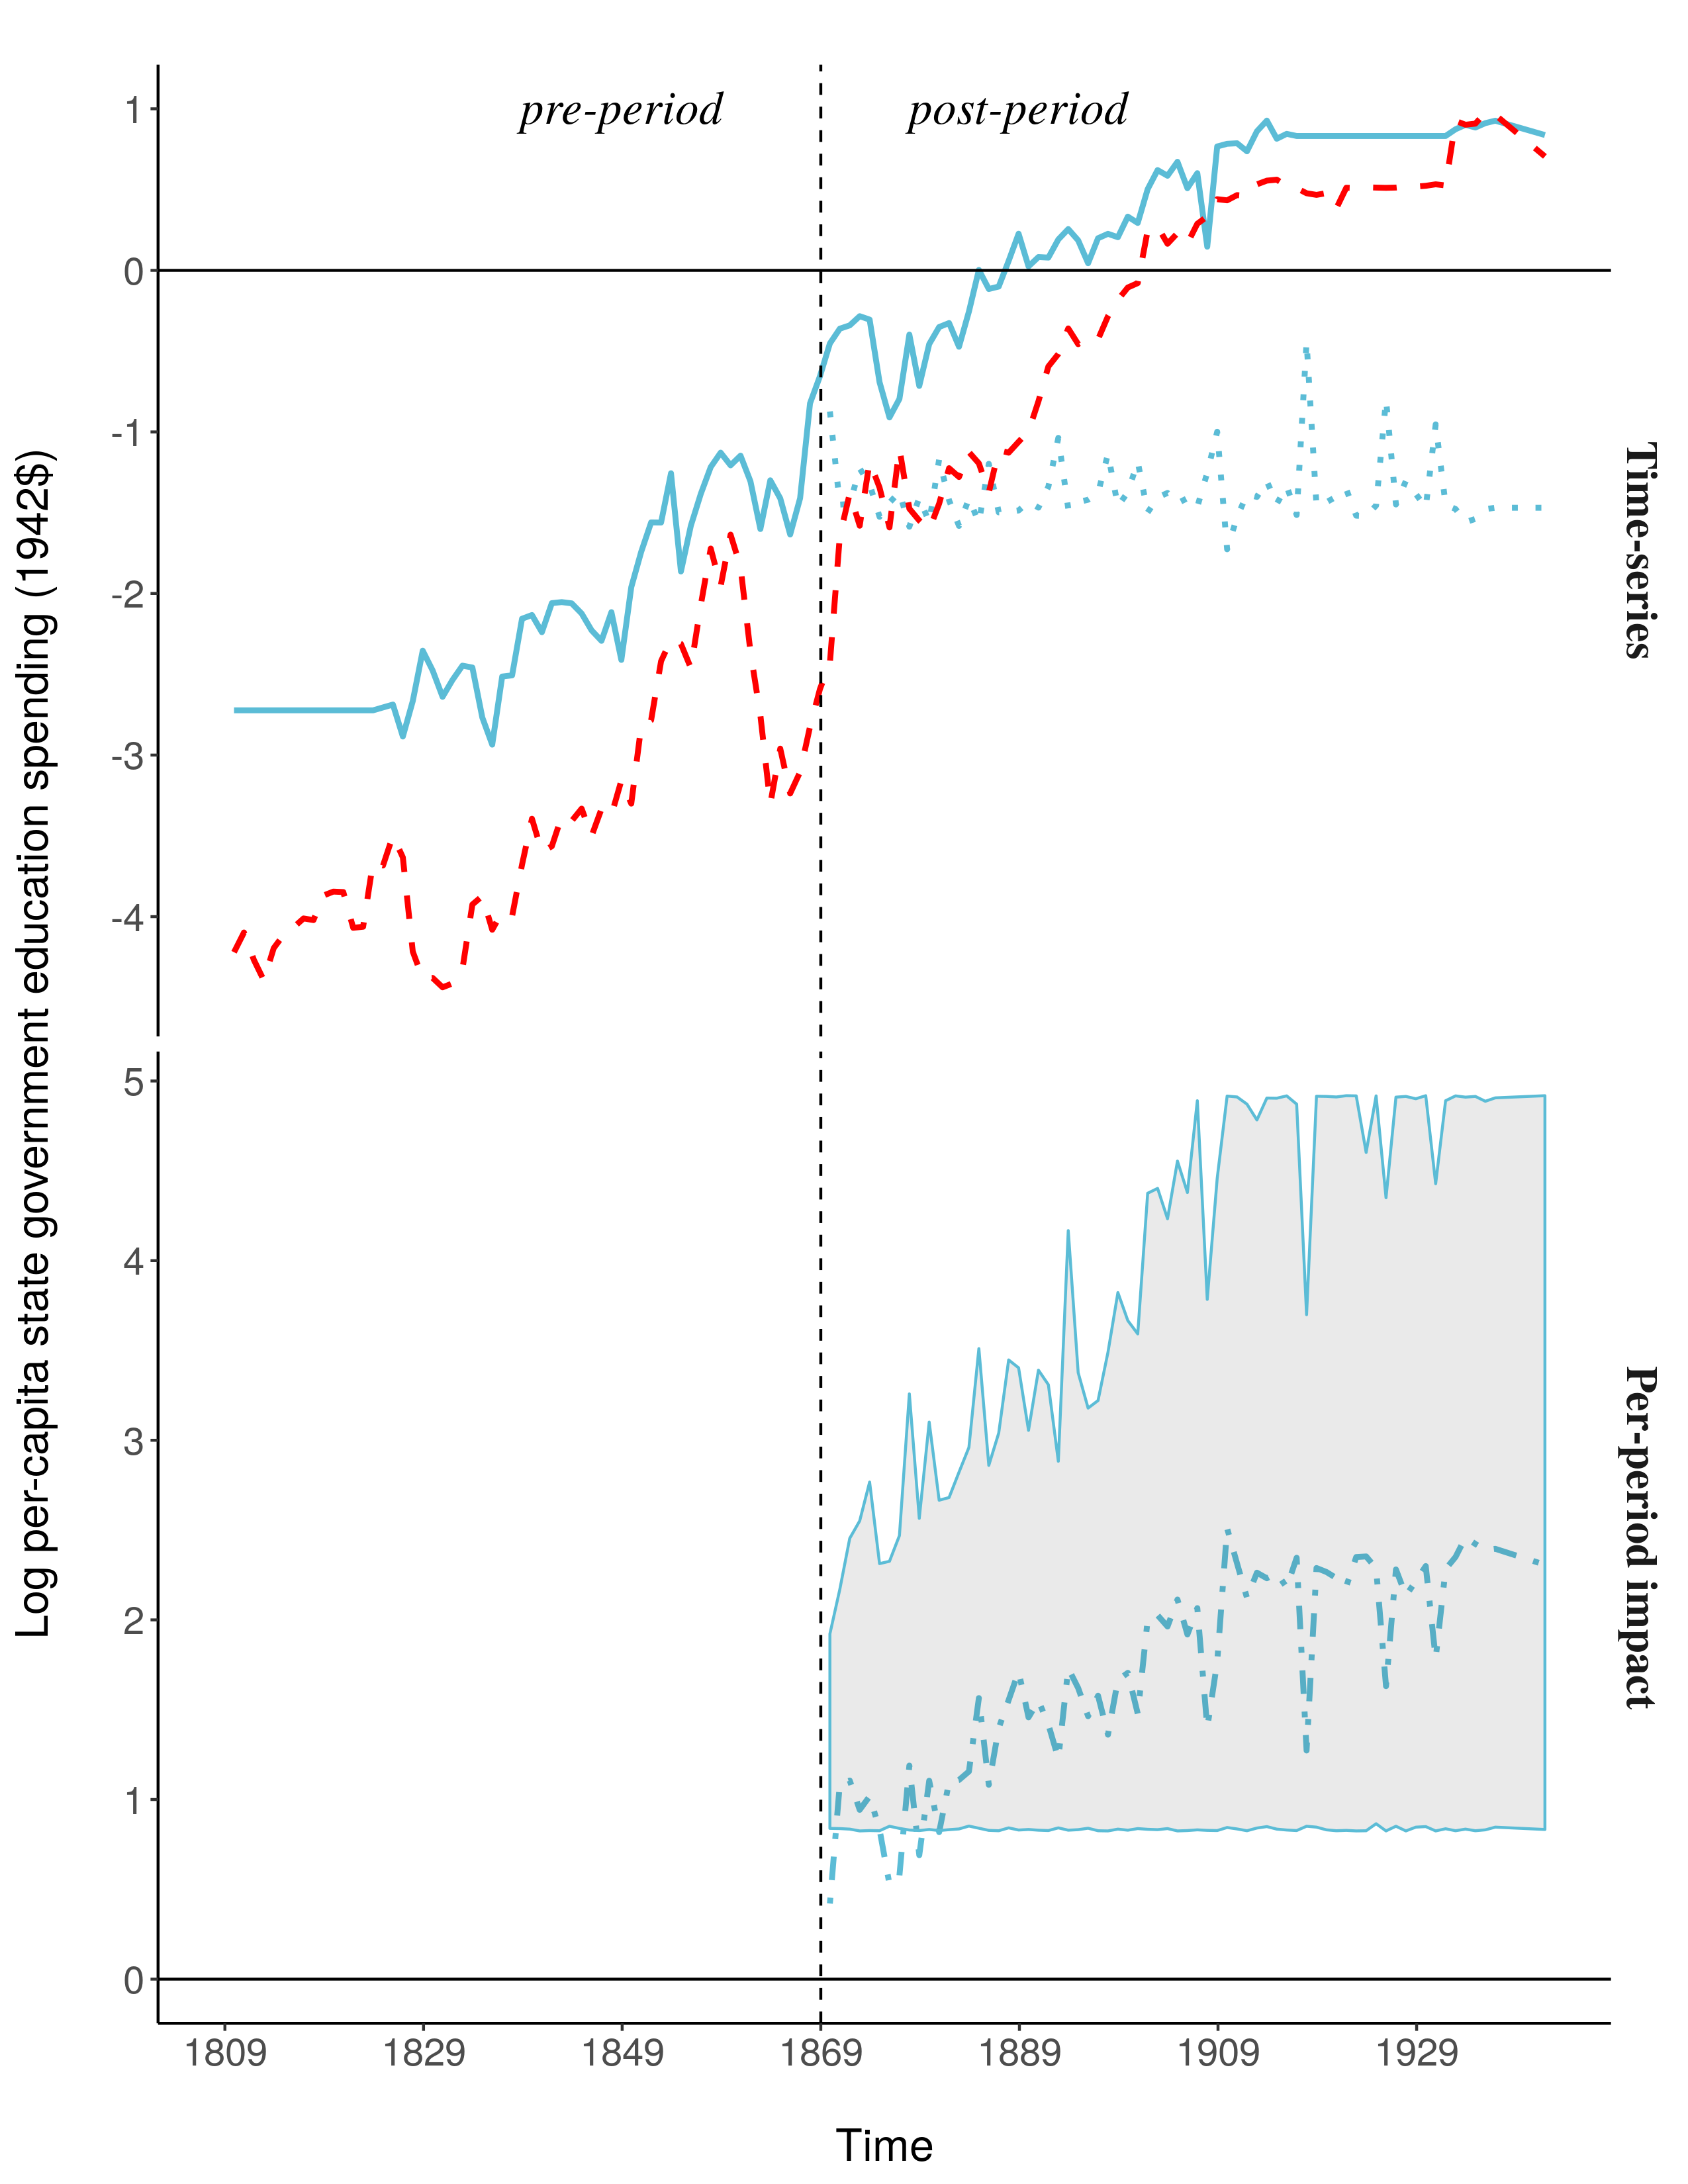
\includegraphics[width=\textwidth]{/media/jason/Dropbox/github/rnns-causal/results/plots/educ-rvae.png}
%	\caption{RVAE estimates of the homestead act on state government education spending, 1809 to 1982.\label{rvae-ed}} 
%\end{figure}

\begin{figure}[htbp]
	\begin{center}
		\includegraphics[width=\textwidth]{/media/jason/Dropbox/github/land-reform/paper/plots/homestead-heatmap.png}
	\end{center}
	\caption{Per-capita homestead entries in state $i$ and year $t$, 1869-1922. \label{fig:homestead-heatmap}}
\end{figure}

\end{appendices}

\itemize
\end{document}